%%%%%%%%%%%%%%%%%%%%%%%%%%%%%%%%%%%%%%%%%
% Beamer Presentation
% LaTeX Template
% Version 1.0 (10/11/12)
%
% This template has been downloaded from:
% http://www.LaTeXTemplates.com
%
% License:
% CC BY-NC-SA 3.0 (http://creativecommons.org/licenses/by-nc-sa/3.0/)
%
%%%%%%%%%%%%%%%%%%%%%%%%%%%%%%%%%%%%%%%%%

%----------------------------------------------------------------------------------------
%	PACKAGES AND THEMES
%----------------------------------------------------------------------------------------

\documentclass{beamer}

\mode<presentation> {

% The Beamer class comes with a number of default slide themes
% which change the colors and layouts of slides. Below this is a list
% of all the themes, uncomment each in turn to see what they look like.

%\usetheme{default}
%\usetheme{AnnArbor}
%\usetheme{Antibes}
%\usetheme{Bergen}
%\usetheme{Berkeley}
%\usetheme{Berlin}
%\usetheme{Boadilla}
%\usetheme{CambridgeUS}
%\usetheme{Copenhagen}
%\usetheme{Darmstadt}
%\usetheme{Dresden}
%\usetheme{Frankfurt}
%\usetheme{Goettingen}
%\usetheme{Hannover}
%\usetheme{Ilmenau}
%\usetheme{JuanLesPins}
%\usetheme{Luebeck}
\usetheme{Madrid}
\usepackage[utf8]{inputenc}
\usepackage[brazilian]{babel}
%\usetheme{Malmoe}
%\usetheme{Marburg}
%\usetheme{Montpellier}
%\usetheme{PaloAlto}
%\usetheme{Pittsburgh}
%\usetheme{Rochester}
%\usetheme{Singapore}
%\usetheme{Szeged}
%\usetheme{Warsaw}

% As well as themes, the Beamer class has a number of color themes
% for any slide theme. Uncomment each of these in turn to see how it
% changes the colors of your current slide theme.

%\usecolortheme{albatross}
%\usecolortheme{beaver}
%\usecolortheme{beetle}
%\usecolortheme{crane}
%\usecolortheme{dolphin}
%\usecolortheme{dove}
%\usecolortheme{fly}
%\usecolortheme{lily}
%\usecolortheme{orchid}
%\usecolortheme{rose}
%\usecolortheme{seagull}
%\usecolortheme{seahorse}
%\usecolortheme{whale}
%\usecolortheme{wolverine}


%\setbeamertemplate{footline} % To remove the footer line in all slides uncomment this line
%\setbeamertemplate{footline}[page number] % To replace the footer line in all slides with a simple slide count uncomment this line

%\setbeamertemplate{navigation symbols}{} % To remove the navigation symbols from the bottom of all slides uncomment this line
}

\usepackage{subfig}
\usepackage{multirow}
\usepackage{hyperref}
\usepackage{graphicx} % Allows including images
\usepackage{booktabs} % Allows the use of \toprule, \midrule and \bottomrule in tables

%----------------------------------------------------------------------------------------
%	TITLE PAGE
%----------------------------------------------------------------------------------------

\title[Defesa de Mestrado]{Análise Digital de Imagens Microtomográficas de \\[0.1cm] Amostras de Reservatórios de Petróleo } % The short title appears at the bottom of every slide, the full title is only on the title page

\author[UNICAMP]{Candidata: Letícia da Silva Bomfim \\ Orientador: Prof. Dr. Hélio Pedrini \\Coorientador: Dr. Guilherme Avansi} % Your name
\institute[]{Universidade Estadual de Campinas \\ Instituto de Computação}
\subtitle{Defesa de Mestrado}
\medskip
%textit{.com} % Your email address

\date{20 de Fevereiro de 2020} % Date, can be changed to a custom date

\titlegraphic{
    \vspace{1cm}
    \hspace{10cm}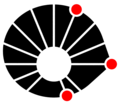
\includegraphics[width=1cm]{fig/logo-unicamp.png}
    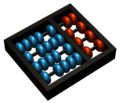
\includegraphics[width=1cm]{fig/logo-ic-unicamp.png}
}

\begin{document}

\begin{frame}
\titlepage % Print the title page as the first slide
\end{frame}

\begin{frame}
\frametitle{Índice} % Table of contents slide, comment this block out to remove it
\tableofcontents % Throughout your presentation, if you choose to use \section{} and \subsection{} commands, these will automatically be printed on this slide as an overview of your presentation
\end{frame}

%----------------------------------------------------------------------------------------
%	PRESENTATION SLIDES
%----------------------------------------------------------------------------------------

%------------------------------------------------
\section{Introdução} % Sections can be created in order to organize your presentation into discrete blocks, all sections and subsections are automatically printed in the table of contents as an overview of the talk
%------------------------------------------------




\begin{frame}{Introdução}{Caracterização do Problema}
\begin{itemize}

\item Necessidade da identificação de um reservatório em potencial e auxílio no processo de tomada de decisão.

\item Uma análise prévia do campo de petróleo pode reduzir os gastos de um projeto e direcionam o seu gerenciamento. 

\item Aplicar análise digital substituindo o método de análise manual.
\begin{itemize}
\item Métodos destrutivos: expansão de gás hélio, injeção de nitrogênio..
\item \textbf{Métodos não destrutivos: análise digital}
\end{itemize}
\end{itemize}

\end{frame}



\begin{frame}{Introdução}{Implicação da Análise Digital}

\begin{itemize}
    \item Preservação das Rochas
    \item Análise profunda e minimalista das estruturas internas.
    
\end{itemize}

\begin{figure}[!htb]
\centering
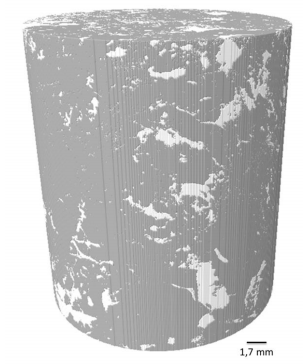
\includegraphics[width=2.5cm]{fig/amostra3d} \\
{\scriptsize Reprsentação digital de uma amostra de rocha.\protect\footnote{Piloto et al. Análise de Imagens de Micro-tomógrafo Digitalizadas para a Caracterização Microestrutural de Carbonatos. 2014}}
\end{figure}

\end{frame}


\begin{frame}{Introdução}{Como é feito este processo?}
    \begin{itemize}
        \item Sondagens e amostragens feitas dos campos em análise.
        \begin{itemize}
            \item O reservatório de petróleo ou zona de produção é uma formação rochosa permeável, porosa ou fraturada.~\protect\footnote{J. E. Thomas. Fundamentos de Engenharia de Petróleo. Interciência, 2001.}
        \end{itemize}
    \end{itemize}
    
    \begin{figure}[!htb]
        \centering
        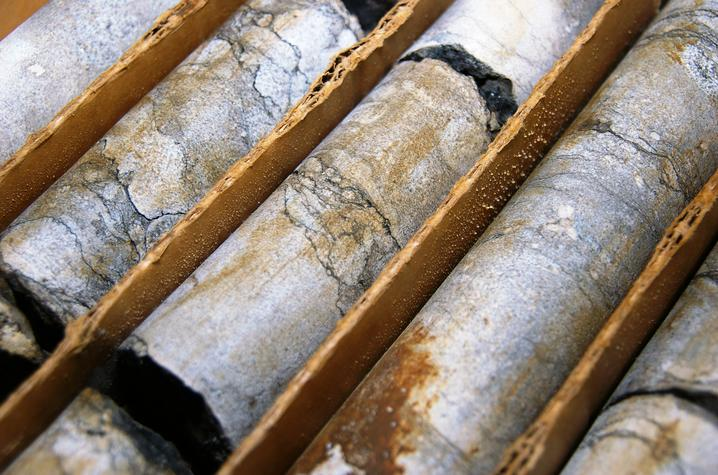
\includegraphics[width=6.5cm]{fig/testemunho.jpg}\\
        {\scriptsize Exemplo de testemunhos rochosos resultantes de sondagens. \protect\footnote{https://uknow.uky.edu/research/federal-grant-will-improve-rock-sample-archives-kentucky-geological-survey}}
    \end{figure}
\end{frame}

\begin{frame}{Introdução}{Aquisição das imagens}
    \begin{itemize}
        \item Técnica de Microtomografia
    \end{itemize}
    
    \begin{figure}[!htb]
        \centering
        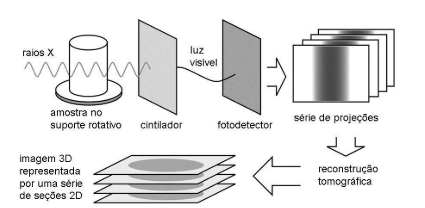
\includegraphics[width=8.5cm]{fig/metodoMRX.PNG}\\
        \scriptsize{Ilustração do processo de aquisição e reconstrução de imagens por tomografia computadorizada~\protect\footnote{D. Uliana, H. Kahn, R. Contessotto, and J. L. Antoniassi. Microtomografia de AltaResolução no Setor Mineral.HOLOS, 3:11–19, 2014}.}
        \label{fig:metodoMRX}
    \end{figure}
\end{frame}

\begin{frame}{Introdução}{Objetivos}

Produzir uma ferramenta que possibilite a geração de dados a respeito das estruturas internas à rochas, através da análise das imagens de MicroCT. Para isso, precisamos realizar:

    \begin{itemize}
        \item Levantamento bibliográfico e estudo das principais técnicas para análise digital dearenitos derivadas de imagens de microtomografia
        \item Extração das estruturas presentes na amostra a partir de uma técnica aprimorada de segmentação
        \item Classificação dos poros e fraturas a partir de suas características morfológicas
    \end{itemize}
    
\end{frame}

\begin{frame}{Introdução}{Hipóteses}
    \begin{itemize}
    
    \item A segmentação por limiarização é suficiente para extrair corretamente as estruturas internas das amostras?
    
    \item Quais as principais características a respeito da geometria das fraturas? É possível caracterizá-las a partir das estruturas extraídas?
    
    \item Qual a melhor maneira de interagir com os resultados obtidos pela caracterização?
    
    \end{itemize}
\end{frame}
%---------------------------------------------
\section{Contextualização}
%---------------------------------------------

\begin{frame}{Contextualização}
    \begin{itemize}
        \item \textbf{Poros}
        \begin{itemize}
            \item Representados por espaços vazios que dependem da forma, arranjo, variação e tamanho dos grãos presentes na rocha.
        \end{itemize}
        \item \textbf{Fraturas}
        \begin{itemize}
            \item Planos ao longo dos quais o estresse causou perda parcial de coesão na rocha.
        \end{itemize}
    \end{itemize}
    
    
    \begin{figure}[!htb]
        \centering
        \subfloat[]{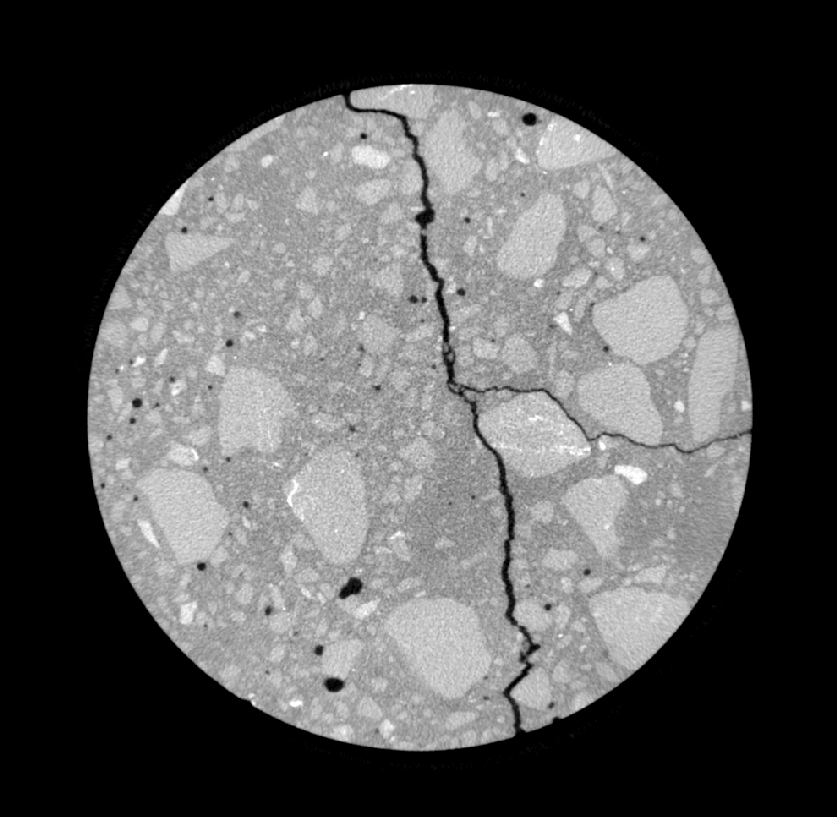
\includegraphics[height=3.0cm]{fig/fratura.png}} \hspace*{0.1cm}
        \subfloat[]{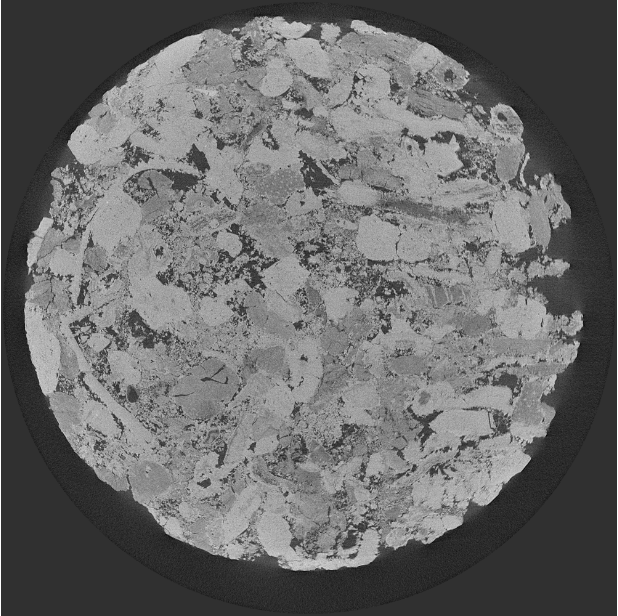
\includegraphics[height=3.0cm]{fig/img_original.png}}\\
         \scriptsize{Exemplos de imagens tomográficas. (a) imagem de rocha carbonática com a presença de uma fratura;~\protect\footnote{A.  du  Plasis.    Concrete  Cracking. 2014} (b) imagem de rocha apenas com poros.~\protect\footnote{T. Bultreys.  Estaillades Carbonate 2, 2016}.}
        \label{fig:microct}
    \end{figure}

\end{frame}

\begin{frame}{Contextualização}{Característica das Estruturas}
   As características permitem a existência do fluxo de fluídos, o que se encontra diretamente ligado a produtividade e lucratividade do reservatório. Algumas delas são:
   
    \begin{table}[]
        \begin{tabular}{c|c}
       \textbf{Poros}         &  \textbf{Fraturas}      \\ \hline
        Porosidade            & Tamanho       \\
        Circularidade         & Conectividade \\
        Visibilidade          & Densidade     \\
        \multicolumn{1}{l|}{} & Orientação   
        \end{tabular}
    \end{table}
\end{frame}

%-------------------------------
\section{Materiais}
%-------------------------------
\begin{frame}{Materiais}{Base de Dados}
    \begin{itemize}
        \item \textit{Digital Rocks Portal}: Um repositório que promove um ambiente de recuperação, armazenamento, compartilhamento, organização e análise de imagens de microestruturas porosas variadas.
        \item Imagens com formato \texttt{.tiff} para facilitar a manipulação dos dados em 2D.
        \item Amostra milimétrica gerando imagens de alta resolução. 
    \end{itemize}
    
\end{frame}

\begin{frame}{Materiais}{Recursos Computacionais}
  \begin{itemize}
      \item \textbf{Principais Ferramentas:}
  \end{itemize}  
    \begin{figure}[!htb]
        \centering
        \subfloat[]{
\includegraphics[height=2cm]{fig/python.png}} \hspace*{0.3cm}
        \subfloat[]{
\includegraphics[height=2.0cm]{fig/opencv.png}}
        \hspace*{0.3cm}
        \subfloat[]{
\includegraphics[height=2.0cm]{fig/VTKlogo.png}} \hspace*{0.3cm}
        \subfloat[]{
\includegraphics[height=2.0cm]{fig/qt-creator-logo.png}} \hspace*{0.3cm}
        \\
         \scriptsize{Ferramentas utilizadas na construção da análise das imagens. (c) Python~\protect\footnote{https://www.python.org/} (d) OpenCV~\protect\footnote{https://opencv.org/} (e) Visualization Toolkit~\protect\footnote{https://vtk.org/} (f) QT Designer~\protect\footnote{https://qt.io/}}
        
    \end{figure}
\end{frame}


%---------------------------------
\section{Metodologia}
%---------------------------------

\begin{frame}{Metodologia}
    \begin{itemize}
        \item Fluxo da metodologia da ferramenta:
    \end{itemize}
    
     \begin{figure}[!htb]
        \centering
        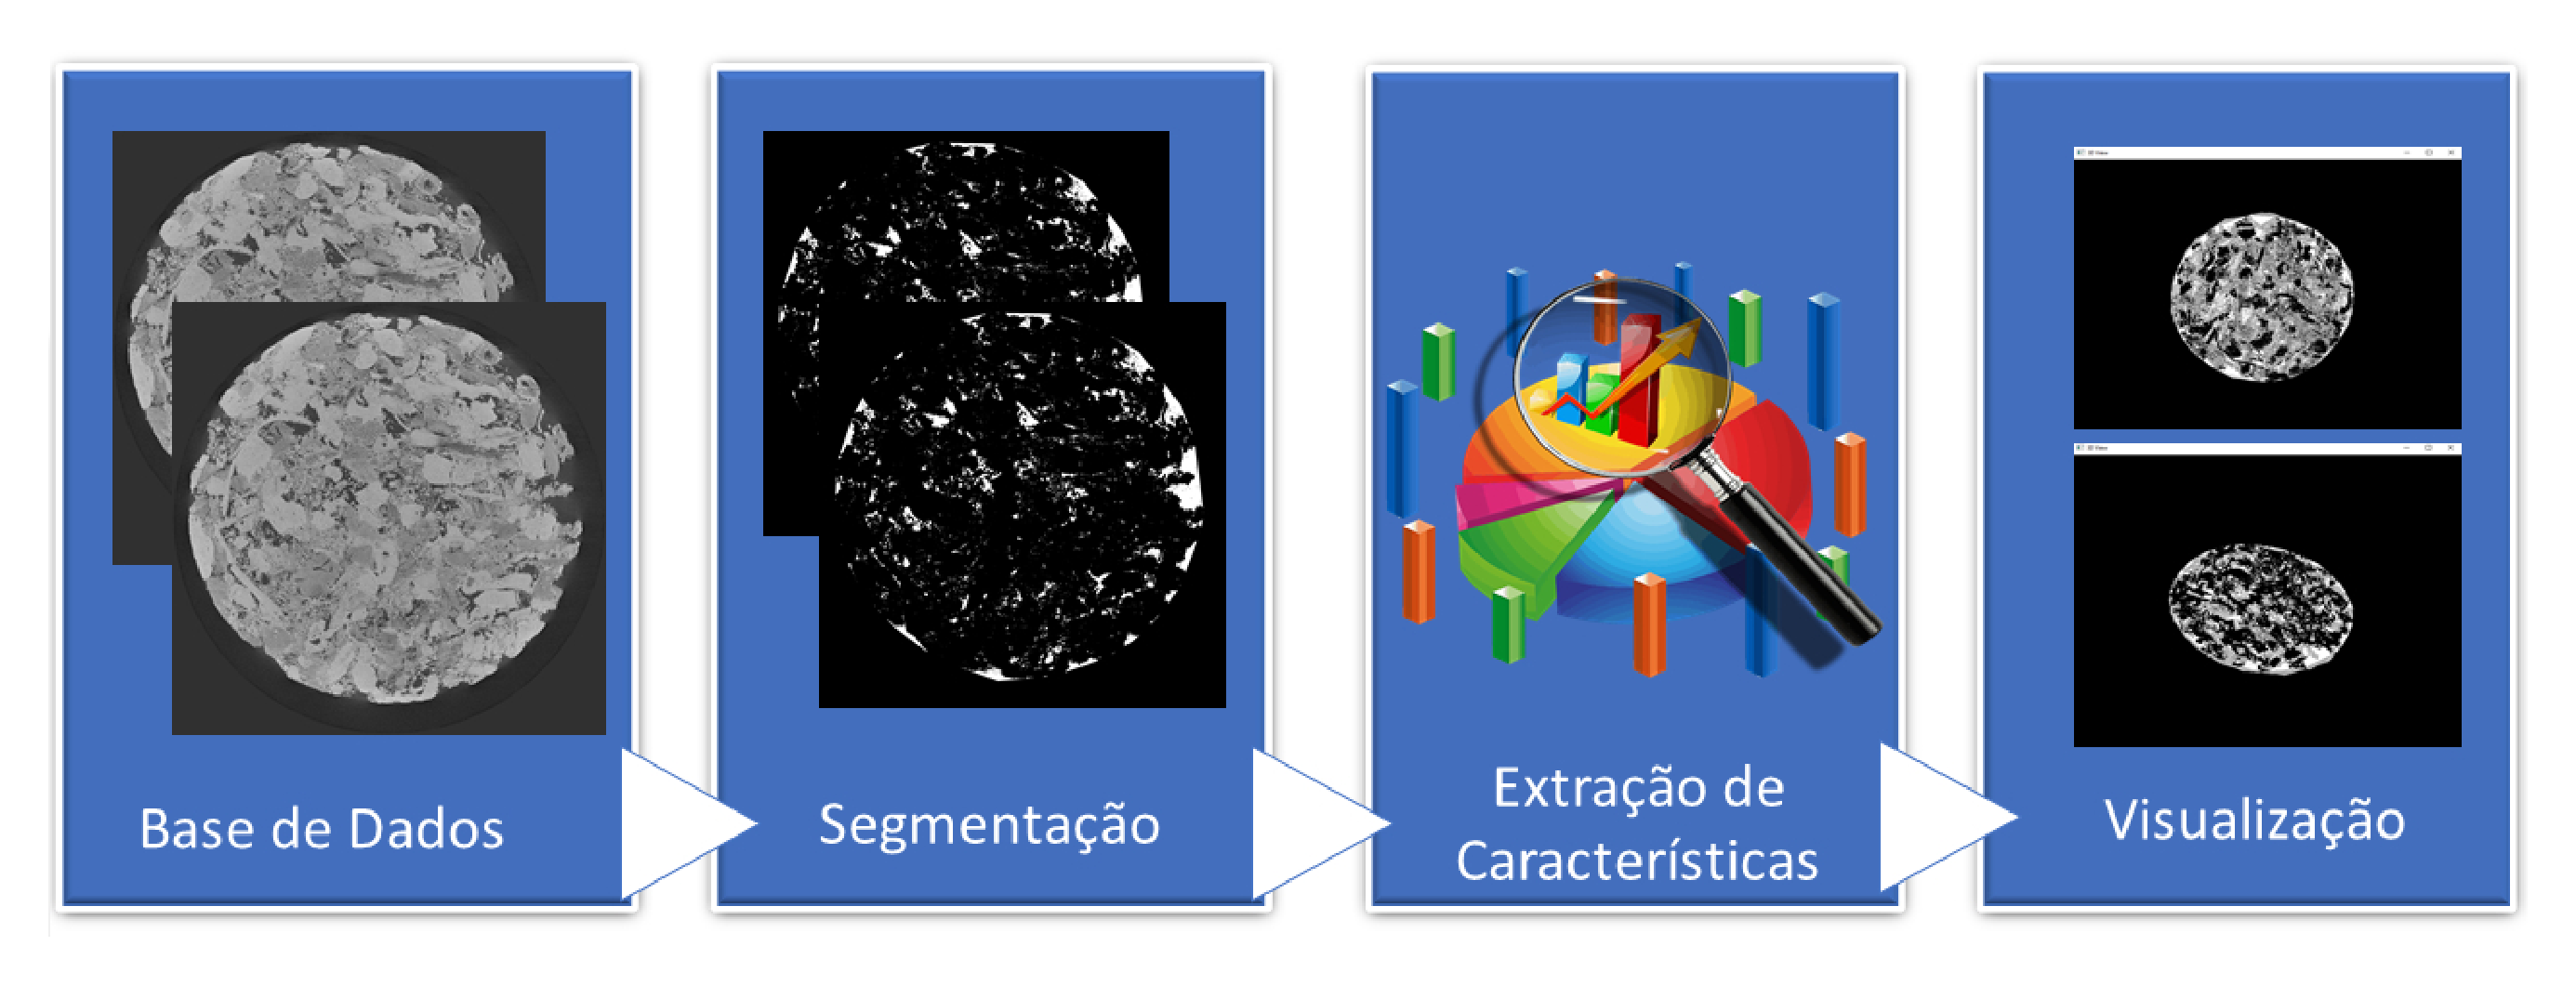
\includegraphics[width=12cm]{fig/descricao.pdf}\\
        \scriptsize{Diagrama da metodologia para análise de estruturas de rochas.}
        \label{fig:metodoMRX}
    \end{figure}
\end{frame}

\begin{frame}{Metodologia}{Segmentação}
 A segmentação é dividade em dois passos:
 \begin{itemize}
     \item A extração da região de interesse.
     \begin{itemize}
        \item Segmentação utilizando principalmente o método de \textit{Watershed}.
        \item Necessidade da aplicação série de técnicas de processamento de imagens. 
    \end{itemize}
    
     \item A extração das estruturas contidas na região de interesse.
     \begin{itemize}
         \item Segmentação utilizando o limiar de Otsu.
         \item Duas análises diferentes: \textbf{Poros e Fraturas}.
     \end{itemize}
 \end{itemize}

\begin{figure}[!htb]
        \centering
        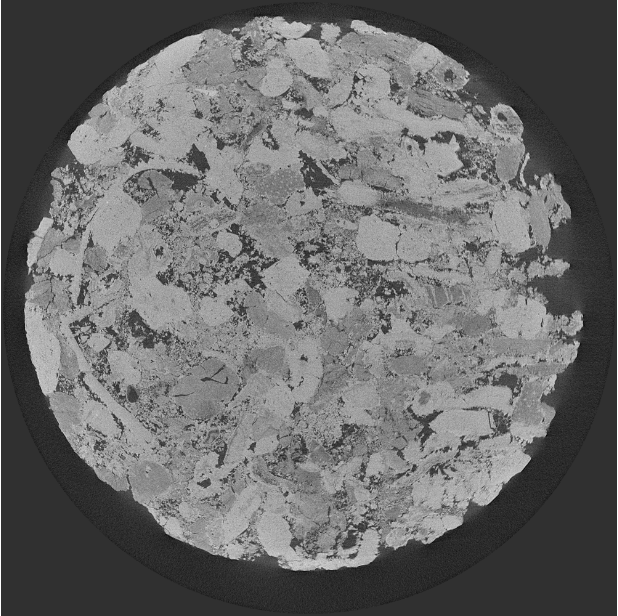
\includegraphics[width=3cm]{fig/img_original.png}
        
\includegraphics[width=3cm]{fig/mask.png}
        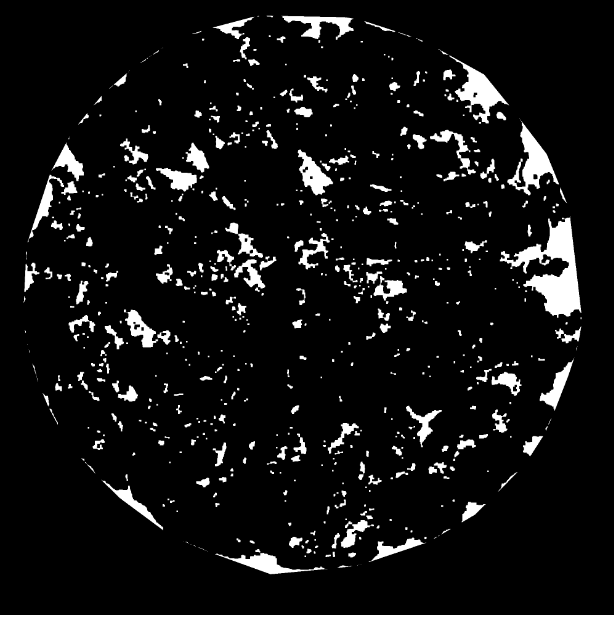
\includegraphics[width=3cm]{fig/seg_final.png}\\
        \scriptsize{Fases da segmentação.}
        \label{fig:metodoMRX}
    \end{figure}
    
\end{frame}

\begin{frame}{Metodologia}{Extração da Região de Interesse.}
    
     \begin{figure}[!htb]
        \centering
        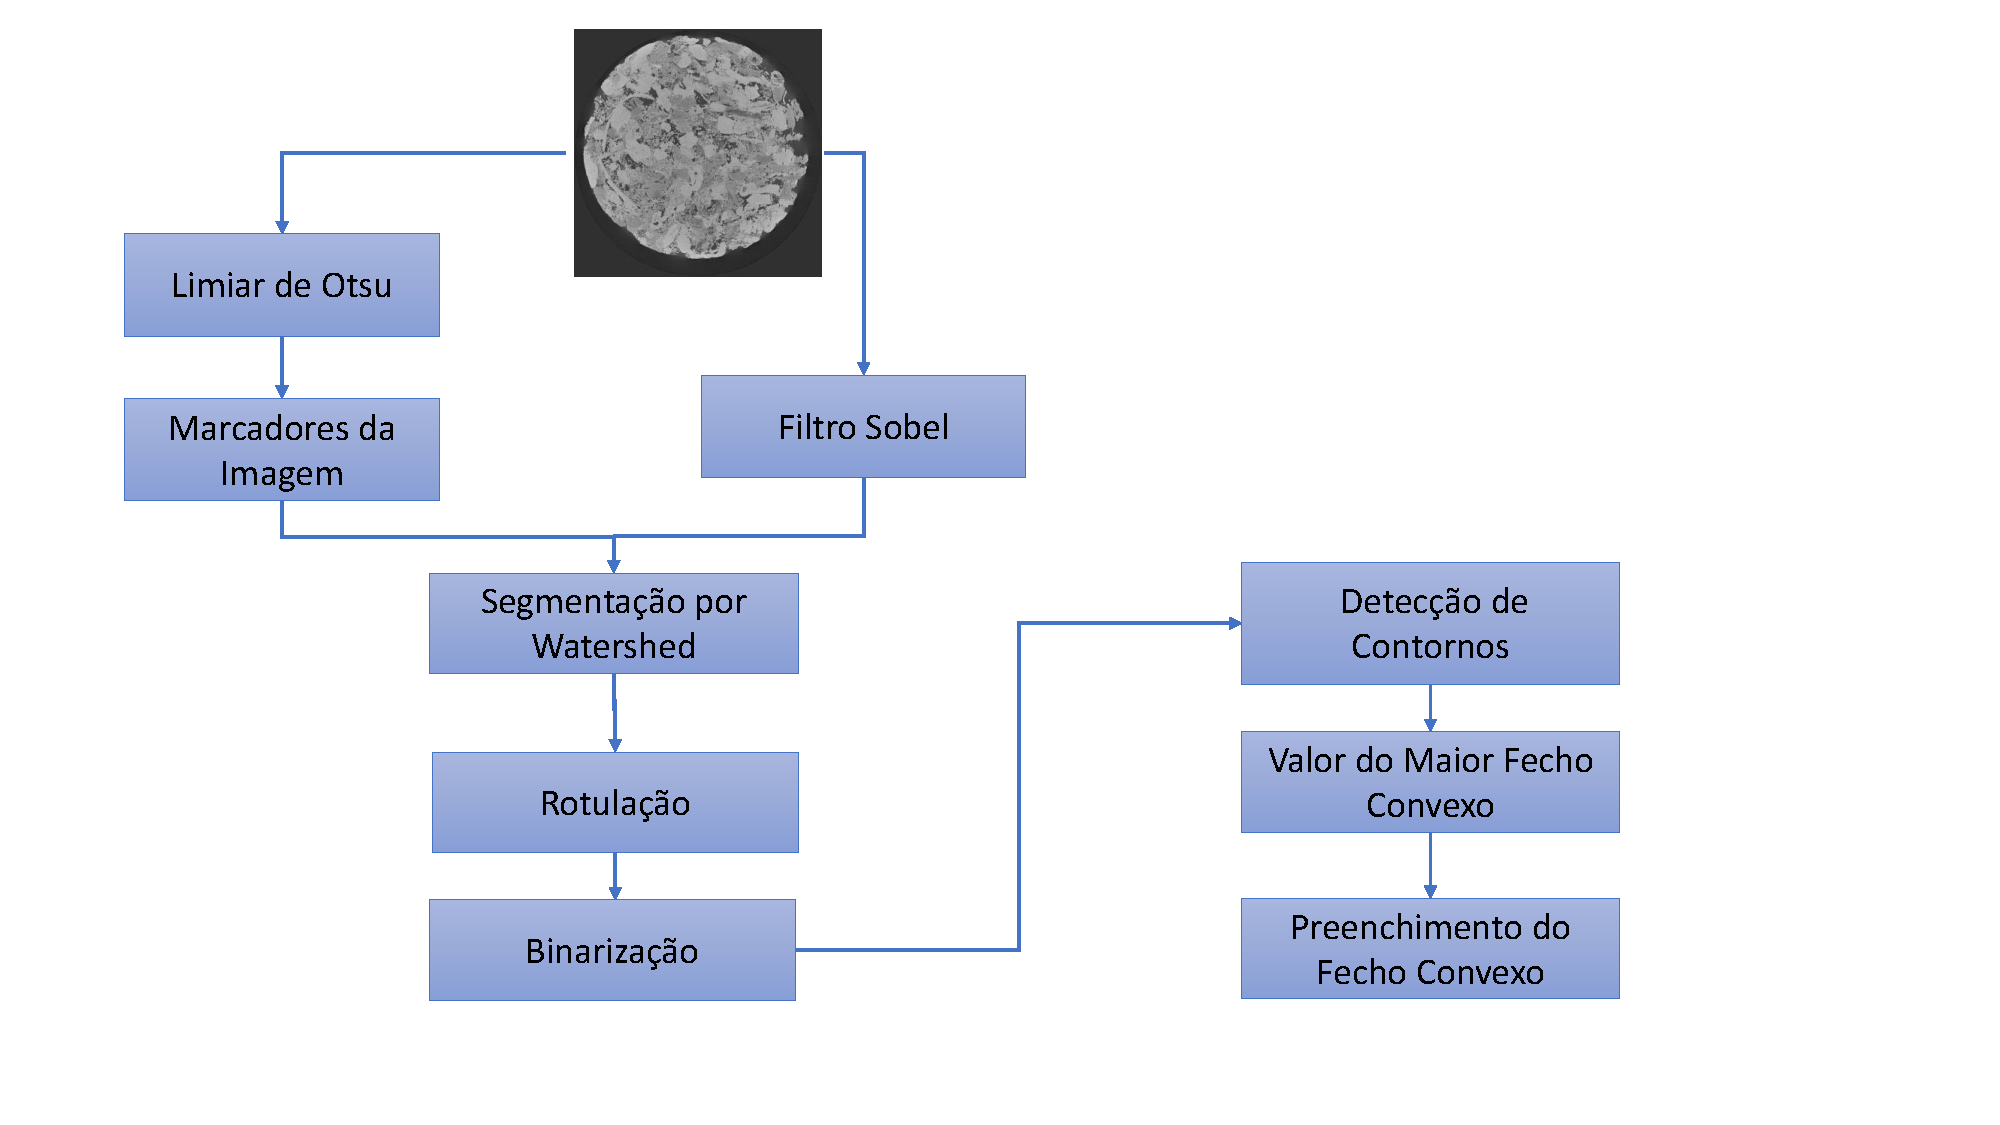
\includegraphics[width=12cm]{fig/mtd-2.pdf}\\
        \scriptsize{Diagrama da metodologia para análise de estruturas de rochas.}
        \label{fig:metodoMRX}
    \end{figure}
    
\end{frame}

\begin{frame}{Metodologia}{Fecho convexo}
    \begin{figure}[!htb]
        \centering
        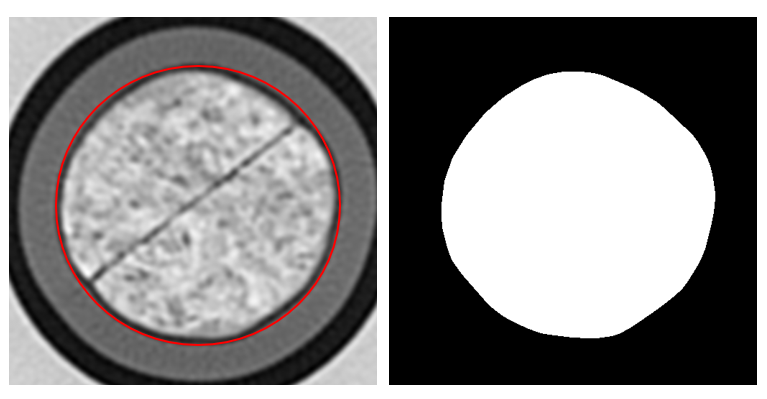
\includegraphics[width=8cm]{fig/ct-sample.png}\\
        \scriptsize{Representação do fecho convexo de interesse e da imagem resultante de sua segmentação.}
        \label{fig:metodoMRX}
    \end{figure}
\end{frame}


\begin{frame}{Metodologia}{Extração das Características das Fraturas}
    O principal passo após a segmentação, neste caso, é a aplicação de técnicas de morfologia matemática que permitam o realce das fraturas.
    \begin{itemize}
        \item \textbf{Operações de Dilatação e Fechamento}
    \end{itemize}
    
    \begin{figure}[!htb]
        \centering
        \subfloat[]{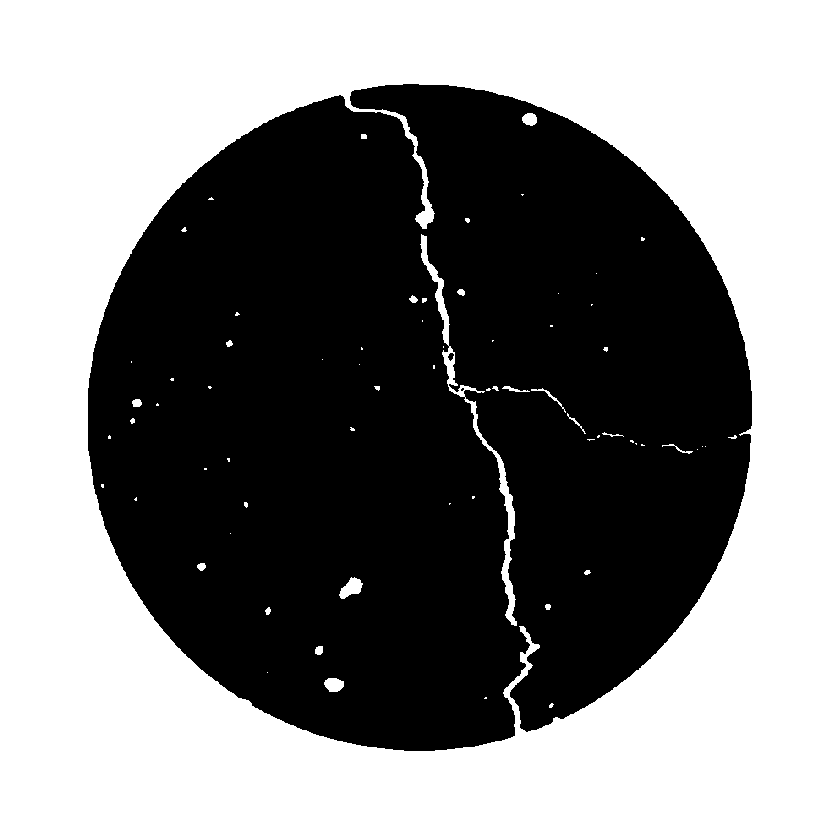
\includegraphics[height=4.0cm]{fig/fratura-thresh.png}} \hspace*{0.2cm}
        \subfloat[]{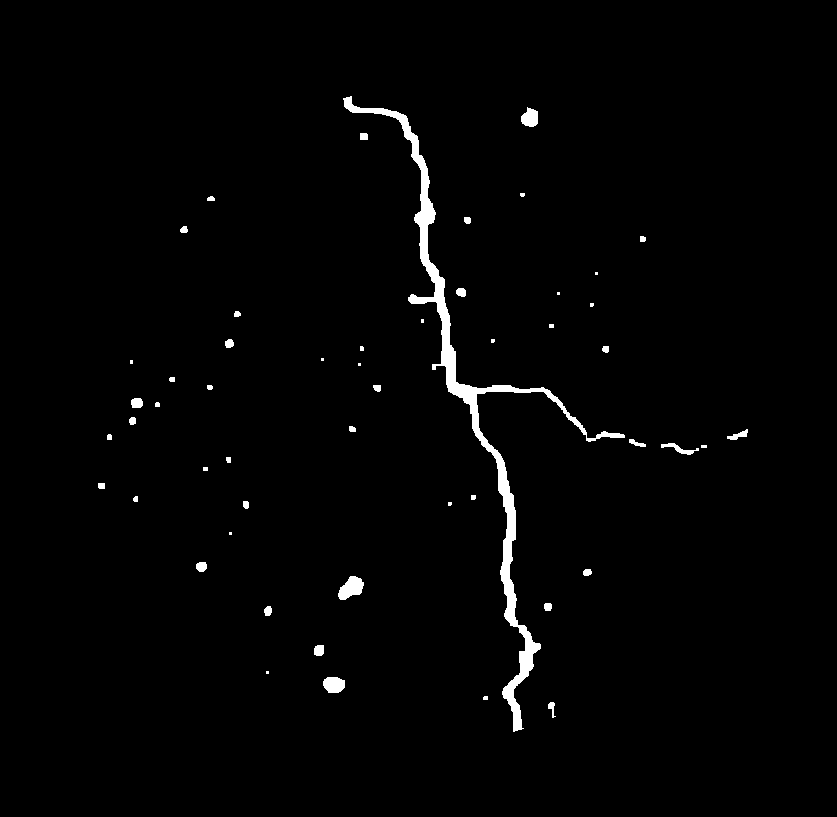
\includegraphics[height=4.0cm]{fig/fratura-seg.png}}\\
        \scriptsize{Pós-processamento da segmentação. (g) imagem segmentada pelo método de Otsu; (h) complementação da segmentação por operações de morfologia matemática.}
    \end{figure}
\end{frame}

\begin{frame}{Metodologia}{Identificação das Fraturas}

\begin{itemize}
    \item Identificação dos contornos que foram extraídos da imagem original a fim de analisar as suas características.
    \begin{itemize}
        \item Uso da função \texttt{findcontours()} da biblioteca \texttt{OpenCV}, essa função auxilia retornando uma lista que contém as descrições de cada estrutura detectada na imagem.
    \end{itemize}
    \item Identificar se os contornos extraídos podem ser classificados como retas.
    \begin{itemize}
        \item Transformada de Hough.
        \item É considerado uma fratura quando se atinge um limiar mínimo de pontos na reta detectada, impedindo que microestruturas sejam extraídas .
    \end{itemize}
\end{itemize}
    
\end{frame}

\begin{frame}{Metodologia}{Angulação}
A angulação é calculada por meio da equação da distância entre dois pontos  $(x_1,y_1)$ e $(x_2,y_2)$ da reta detectada.

\begin{figure}[!htb]
    \centering
    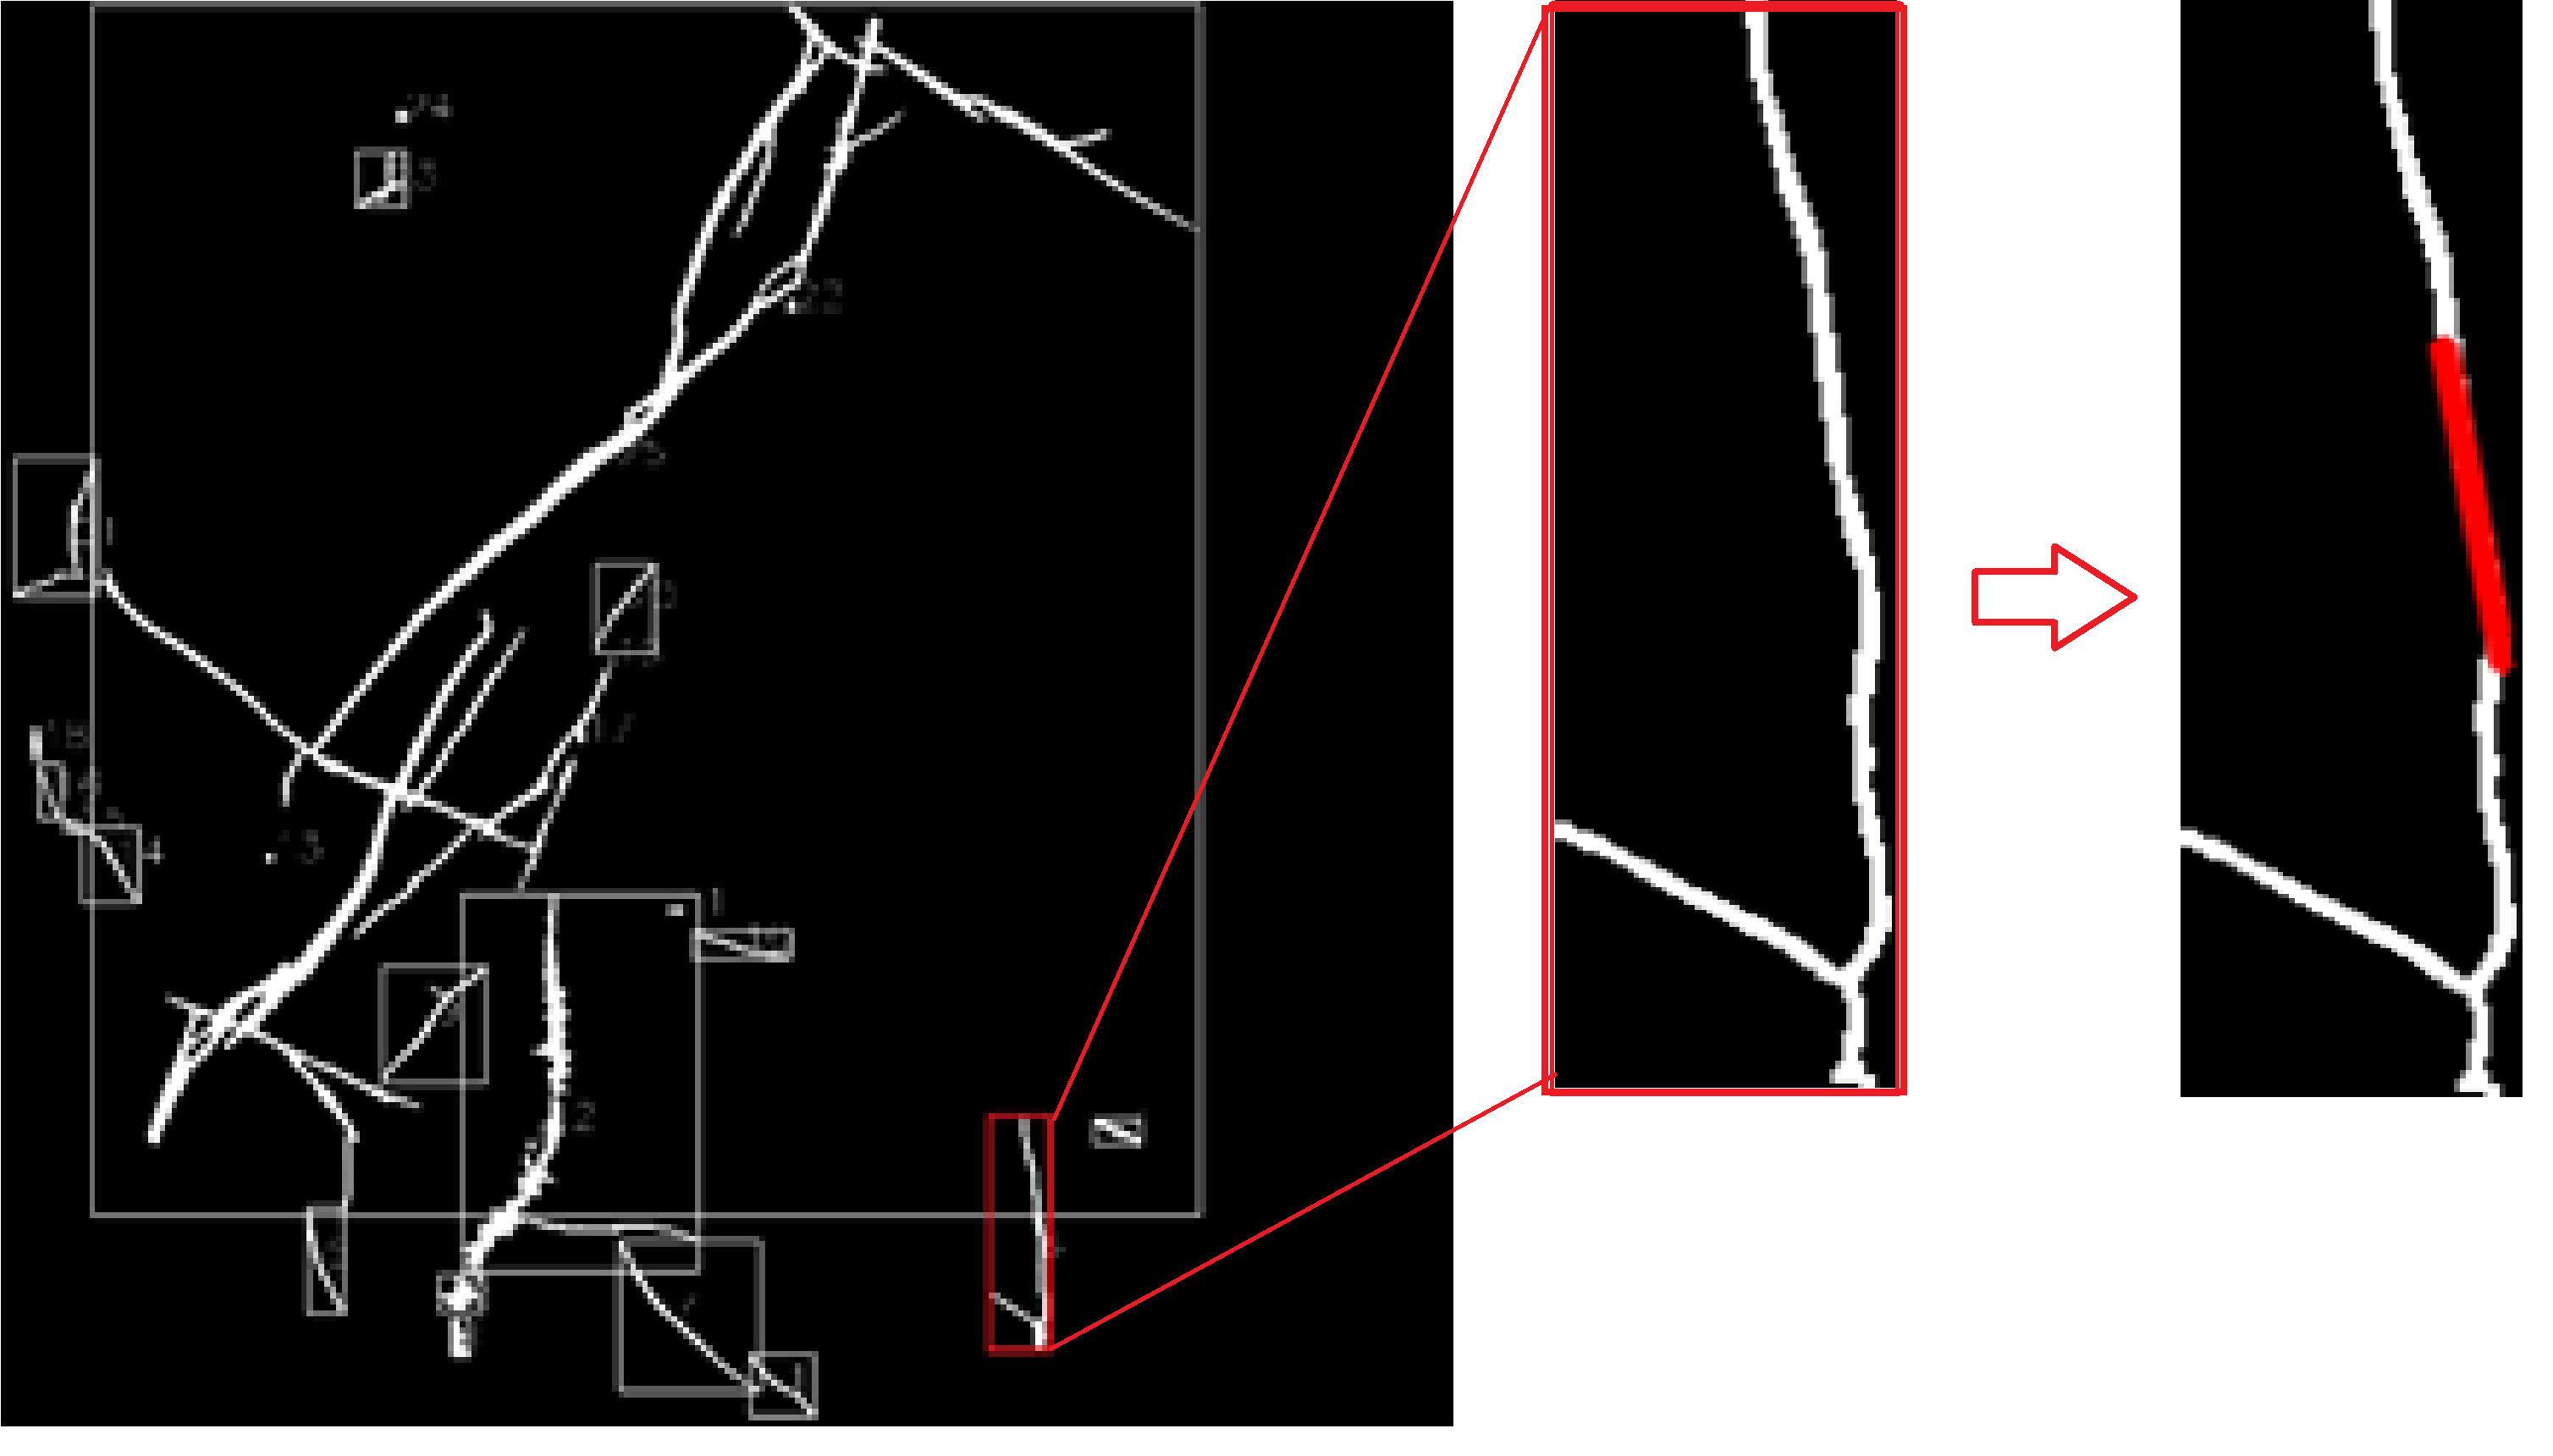
\includegraphics[width=8.5cm]{fig/hough_lines.png}\\
    \scriptsize{Detecção de linhas pela transformada de Hough.}
\end{figure}
    
\end{frame}

\begin{frame}{Metodologia}{Tamanho}

As medidas com respeito ao tamanho são calculadas através dos valores obtidos pelo retângulo envolvente rotativo dos contornos.

\begin{figure}[!htb]
\centering
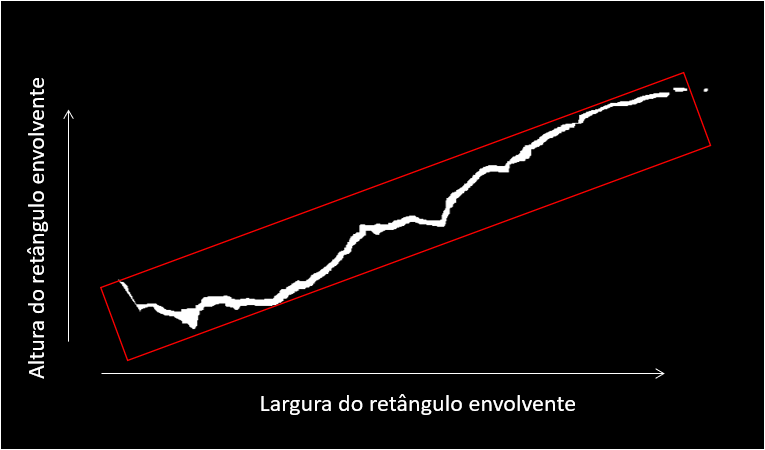
\includegraphics[width=8.0cm]{fig/shape_fracture.PNG}\\
\scriptsize{Ilustração das medidas do retângulo envolvente em relação à fratura.}
\end{figure}

Funções do \texttt{OpenCV} auxiliam a extrair informações como altura e largura.
\end{frame}

\begin{frame}{Metodologia}{Densidade}

\begin{itemize}
    \item Para a densidade linear, utilizou-se o número de fraturas pelo diâmetro da amostra de rocha, sendo:
    \begin{equation}
        d_1 = \frac{\textit{número de fraturas}}{\textit{diâmetro}}
    \end{equation}
    
    
    \item Na densidade 2D, o cálculo é efetuado pela média da largura das fraturas dividido pela área total da amostra, sendo:
    \begin{equation}
        d_2 = \frac{\textit{média(largura das fraturas)}}{\textit{área total da amostra}}
    \end{equation}
    
    \item A densidade 3D, que calcula a relação da área das fraturas pela área da amostra, é dado por:
    \begin{equation}
        d_3 = \frac{\textit{área total das fraturas}}{\textit{área total da amostra}}
    \end{equation}
    
\end{itemize}

\end{frame}

\begin{frame}{Metodologia}{Conectividade: Tipo I,II,II}
    
    \begin{itemize}
        \item \textbf{Processo Inicial:}
        \begin{itemize}
            \item Extração da imagem correspondente ao retângulo envolvente.
            \item Varredura das linhas da imagem resultante.
        \end{itemize}
    \end{itemize}
    
    \begin{figure}[!htb]
    \centering
    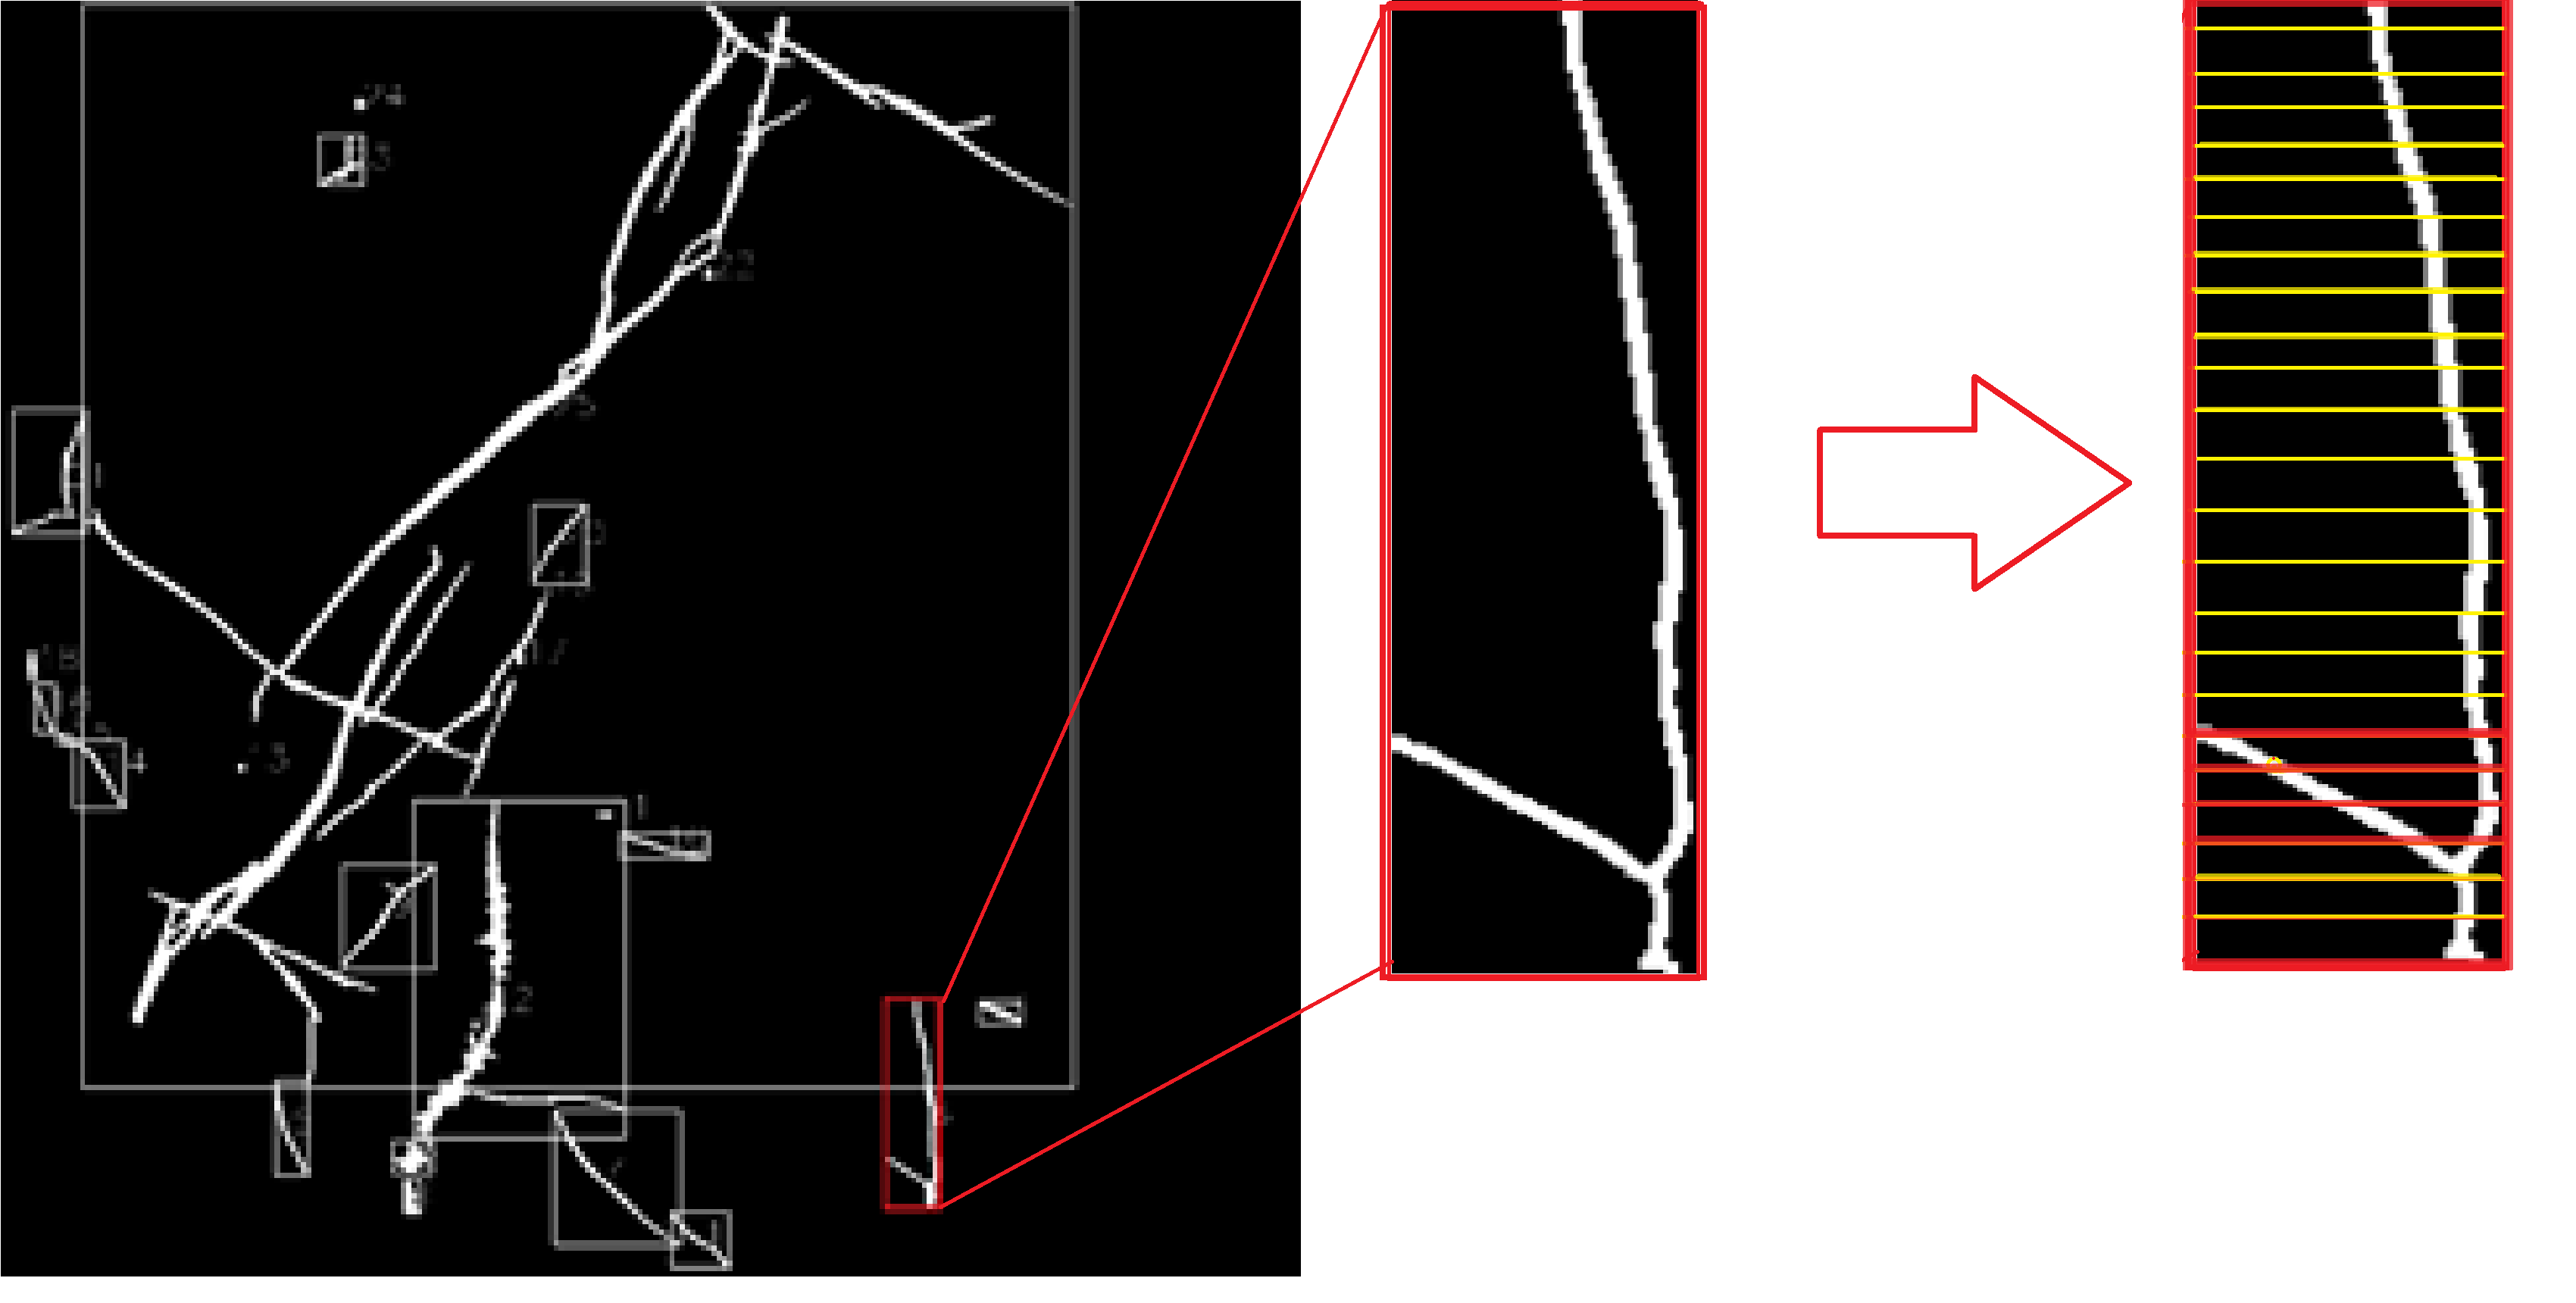
\includegraphics[width=10cm]{fig/conect.png}\\
    \scriptsize{Processo de identificação de bifurcações na fratura.}
    \end{figure}
        

\end{frame}

\begin{frame}{Metodologia}{Conectividade: Tipo I,II,II}
    \begin{itemize}
        \item \textbf{Processo Secundário:}
        \begin{itemize}
        \item Aplicação do método de componentes conexos.
        \item Varredura das linhas da imagem resultante.
    \end{itemize}
    \end{itemize}
    
    
    \begin{figure}[!htb]
    \centering
    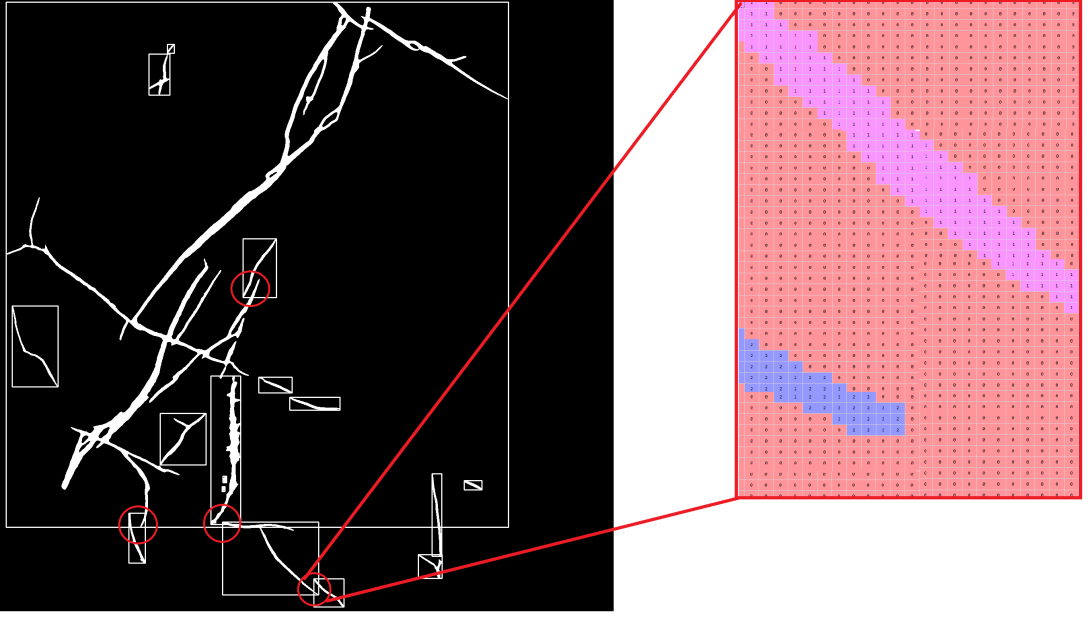
\includegraphics[width=8cm]{fig/conectividade.png}\\
    \scriptsize{Identificação de componentes externos no retângulo envolvente de uma fratura.}
    \label{fig:conectividade}
    \end{figure}

\end{frame}


\begin{frame}{Metodologia}{Conectividade: Sistemática x Não Sistemática}
    \begin{itemize}
        \item Análise do padrão das fraturas sistemáticas.
           \begin{itemize}
               \item Segmentação com maior tolerância a ruídos afim de capturar o comportamento da fraturas menores.
           \end{itemize}
       
    \end{itemize}    
    
    \begin{figure}[!htb]
    \centering
    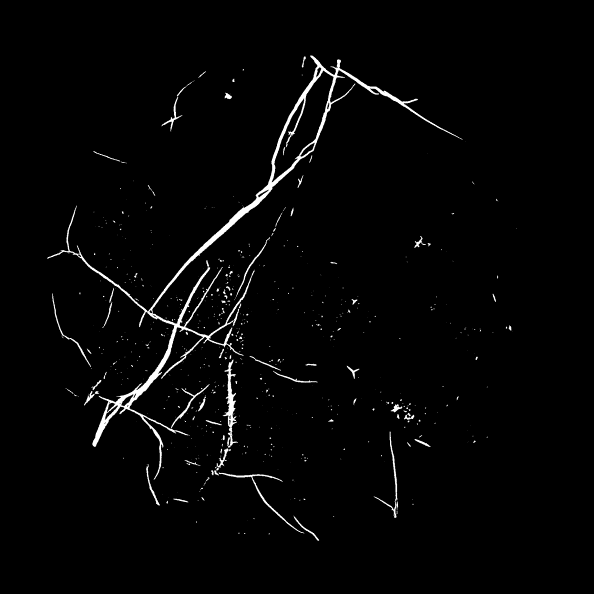
\includegraphics[width=4.5cm]{fig/seg_ruidos.png}\\
    \scriptsize{Imagem segmentada com maior tolerância a ruídos.}
    \end{figure}

\end{frame}    

\begin{frame}{Metodologia}{Conectividade: Sistemática x Não Sistemática}
    
    \begin{itemize}
        \item  Calculo de um limiar para caracterizar uma fratura em sistemática ou não sistemática pela média das larguras das fraturas da fatia, com base nos dados apresentados pelo gráfico.
    \end{itemize}    
    
    \begin{figure}[!htb]
    \centering
    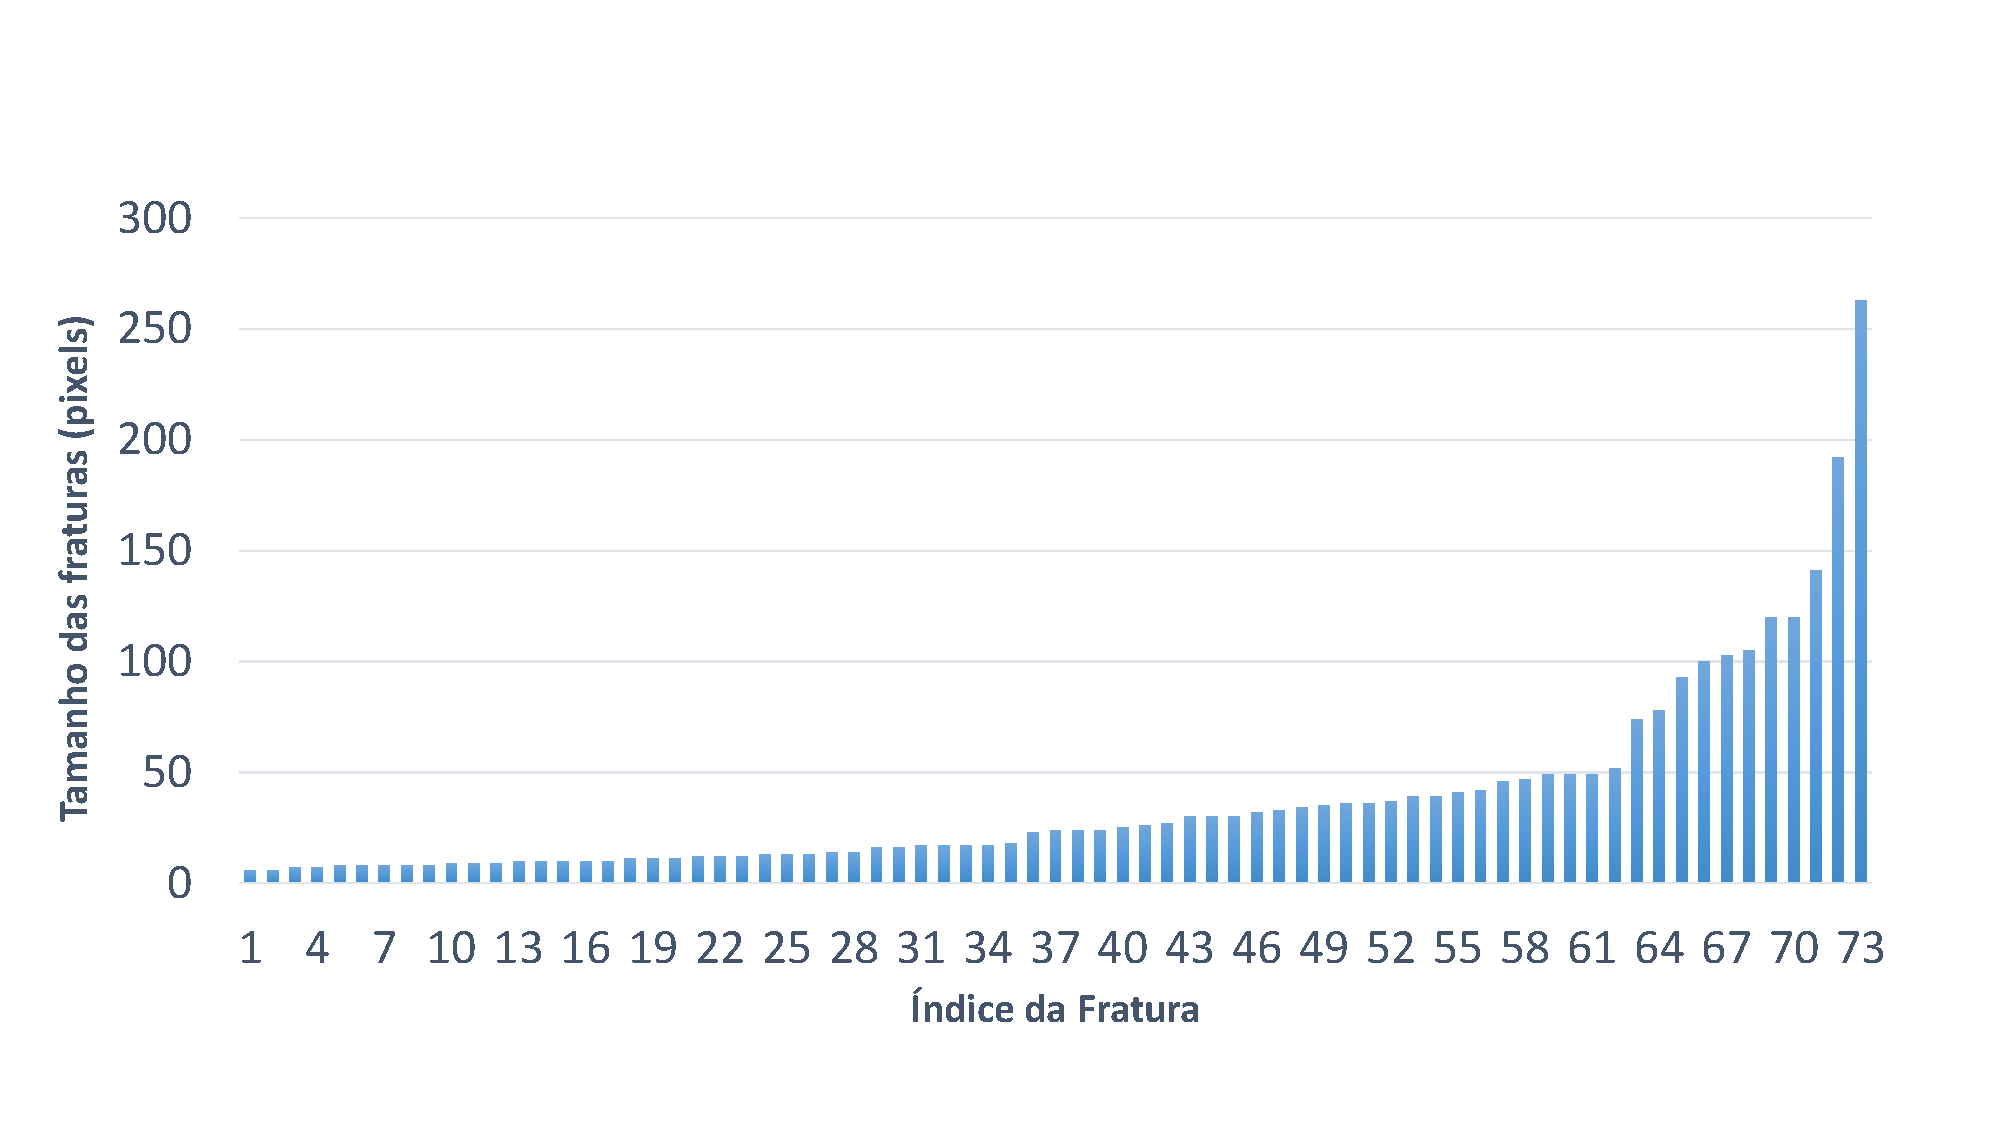
\includegraphics[width=9.5cm]{fig/grafico-distribuicao.pdf}\\
    \scriptsize{Gráfico da distribuição da largura de todas as fraturas de uma mesma fatia.}
    \end{figure}

\end{frame}

\begin{frame}{Metodologia}{Extração das Características dos Poros}
    \begin{itemize}
         
        \item \textbf{Porosidade} calculada pela razão entre o volume dos poros e o volume total da rocha, com o uso da função \texttt{contourArea()}.
        \item \textbf{Circularidade} obtida através da equação:
        \begin{equation}
            \textit{circularidade} = \frac{4\pi \, \textit{área}}{\textit{perímetro}^{2}}
        \end{equation}
        com o uso das equações \texttt{arcLength()} e \texttt{minEnclosingCircle()}.
        \item \textbf{Visibilidade}, classificada por Archie\footnote{G. E. Archie. Classification of Carbonate Reservoir Rocks and Petrophysical Conside-rations.American Association of Petroleum Geologists (AAPG) Bulletin, 36(2):278–298, 1952} em quatro categorias:
                    
        \begin{itemize}
            \item Classe A: não visível, menor que 1 micrômetro.
            \item Classe B: visível, com poros entre 1 e 10 micrômetros.
            \item Classe C: visível, com poros maiores do que 10 micrômetros.
            \item Classe D: \textit{vugs}, com poros maiores do que 1 milímetro.
        \end{itemize}
        
    \end{itemize}
\end{frame}

\begin{frame}{Metodologia}{Visualização}
    
    \begin{itemize}
        \item Propõe uma visualização completa das imagens segmentadas afim de auxiliar na compreensão da distribuição das estruturas de interesse.
    \end{itemize}
    
    \begin{figure}[!htb]
        \centering
        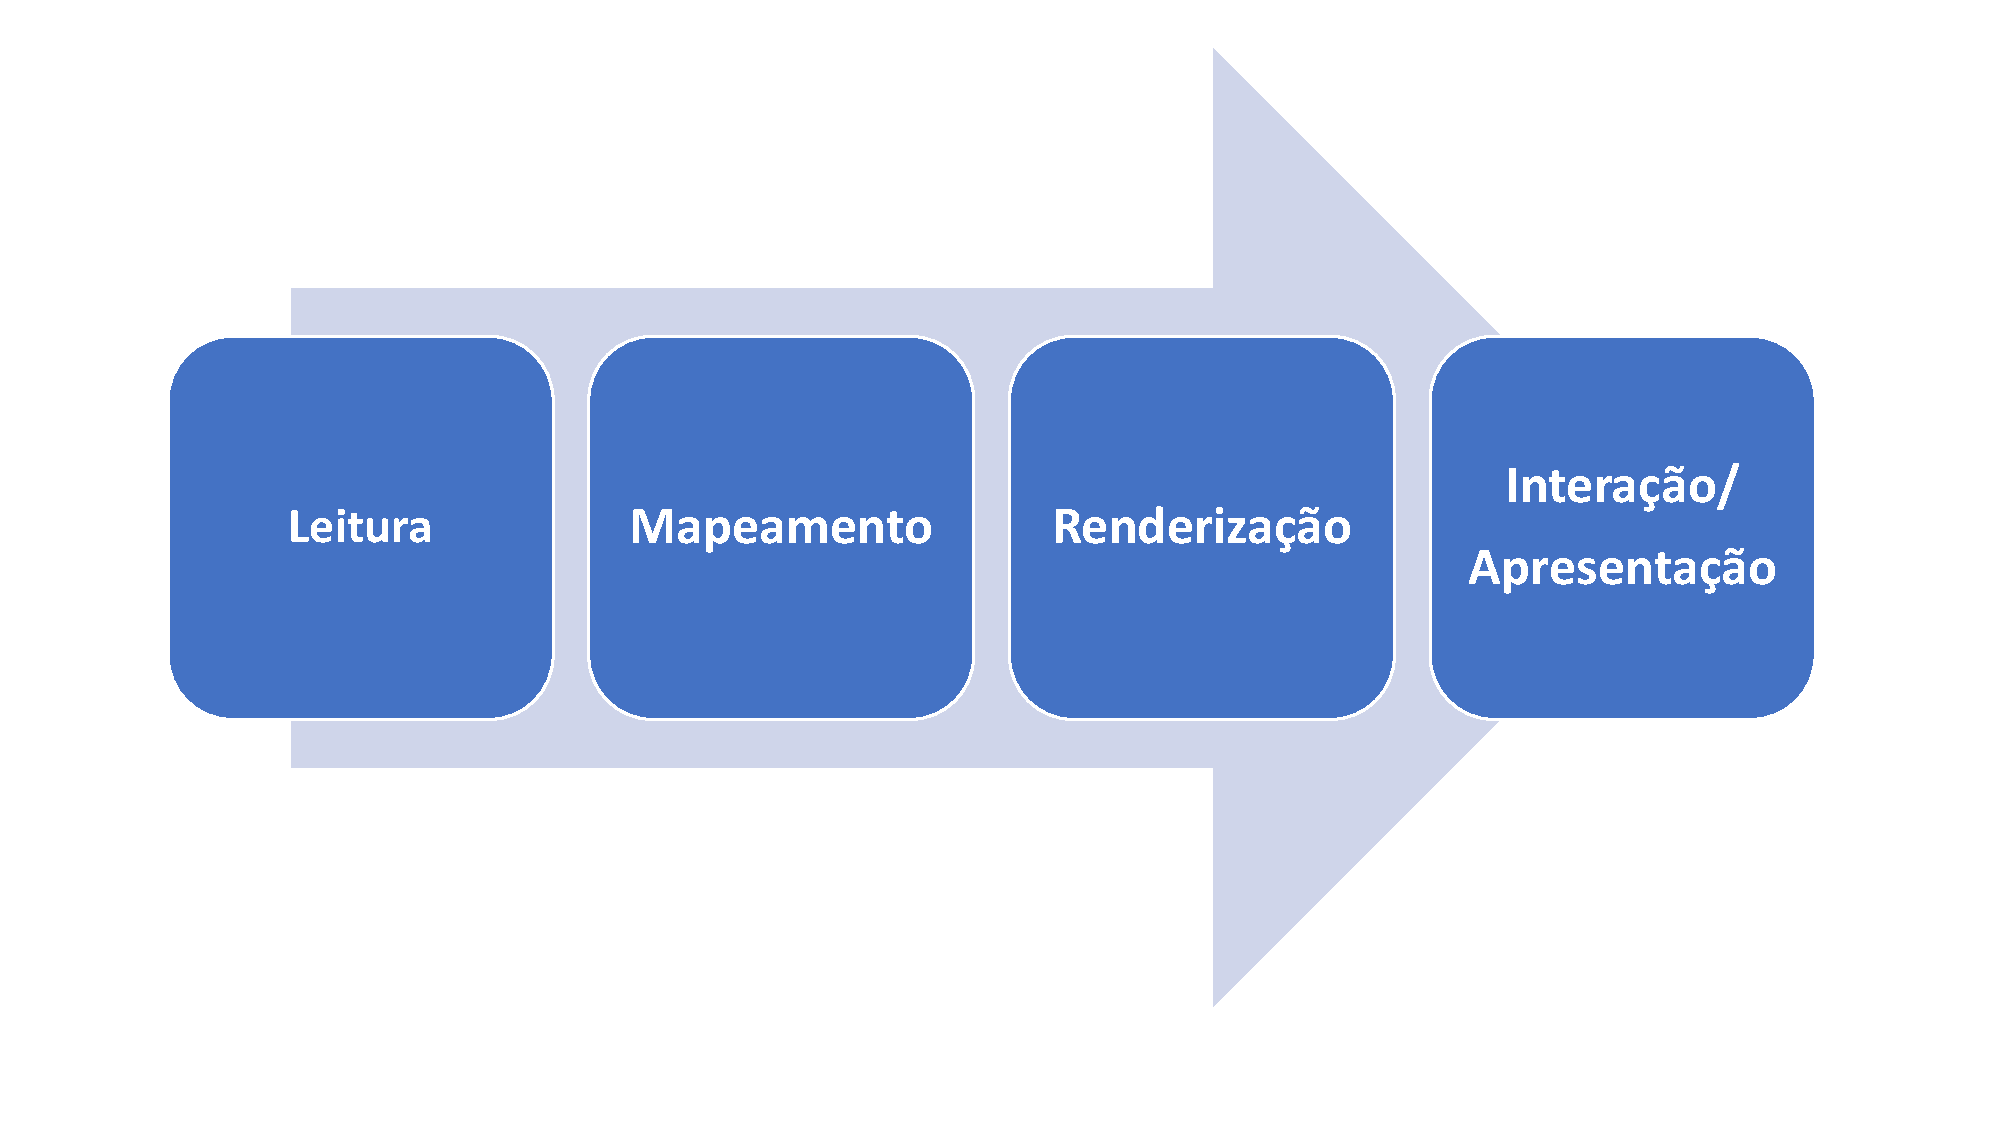
\includegraphics[width=.7\textwidth]{fig/fases_vtk.pdf} \\
        \scriptsize{Fluxo da construção do modelo de visualização.}
    \end{figure}
\end{frame}

%------------------------------------
\section{Resultados Experimentais}
%------------------------------------

\begin{frame}{Resultados Experimentais}{Análise das Características}
    
    \begin{itemize}
        \item Testes iniciais:
    \end{itemize}
        
    \begin{figure}[!htb]
    \centering
    \subfloat[]{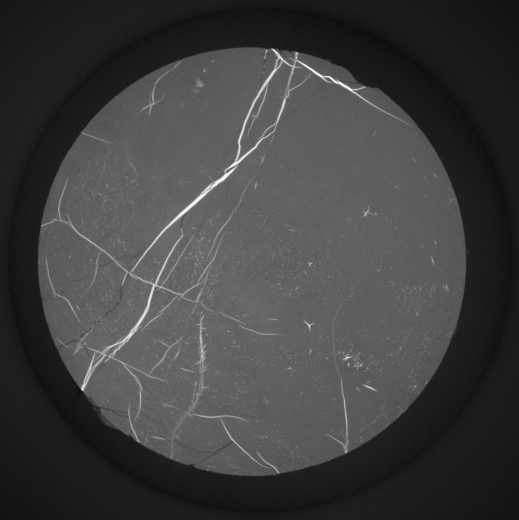
\includegraphics[height=5.0cm]{fig/coal.png}} \hspace*{0.1cm}
    \subfloat[]{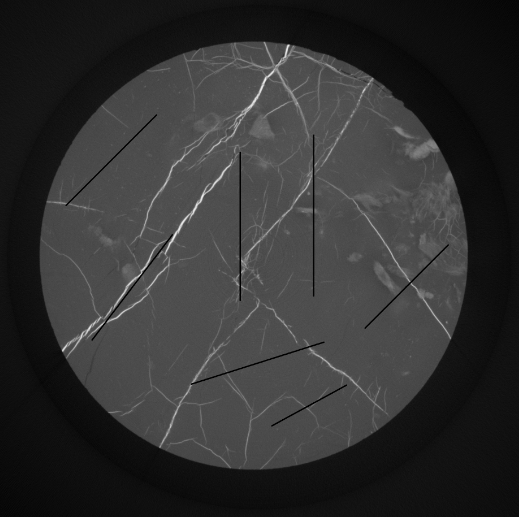
\includegraphics[height=5.0cm]{fig/sintetica.png}}\\
    \scriptsize{Imagens para testes de fraturas. (i) imagem de amostra de carvão; (j) imagem de amostra de carvão com adição de fraturas sintéticas.}
    \label{fig:img_testes}
    \end{figure}
\end{frame}

\begin{frame}{Resultados Experimentais}{Primeiros Resultados}
    \begin{itemize}
    \item Resultados com amostras simples, contendo fraturas do tipo I - não sistemáticas.
    \item Acerto de 100\% quanto ao quesito da análise do seu tipo, centroide e angulação.
    \end{itemize}
    
        
    \begin{table}[!htb]
    \setlength{\tabcolsep}{2.0mm}
    \centering
    \caption{Resultado da análise de fraturas da imagem sintética.}
    \label{tab:resul_sintetico}
    \begin{tabular}{rrrcrr}
    \toprule
    Centroide $X$ & Centroide $Y$ & Ângulo & Tipo & Comprimento & Largura \\
    \midrule
    1097 & 1445 & 30 & I & 307 &   7 \\
     915 & 1295 & 19 & I & 497 &   7 \\
    1442 & 1024 & 46 & I & 475 &   7 \\
     471 & 1027 & 54 & I & 475 &   7 \\
     853 &  811 & 90 & I &   6 & 530 \\
    1113 &  773 & 90 & I &   6 & 574 \\
     397 &  577 & 46 & I & 459 &   7 \\
    \bottomrule
    \end{tabular}
    \end{table}
\end{frame}

\begin{frame}{Resultados}{Análise das Características: Fraturas}
   
    \begin{itemize}
        \item A fim de analisar fraturas mais complexas, utilizamos as imagens da amostra de carvão com calcificação e modificamos as fraturas em branco para preto.
    \end{itemize}
    
    \begin{figure}[!htb]
    \centering
    \subfloat[]{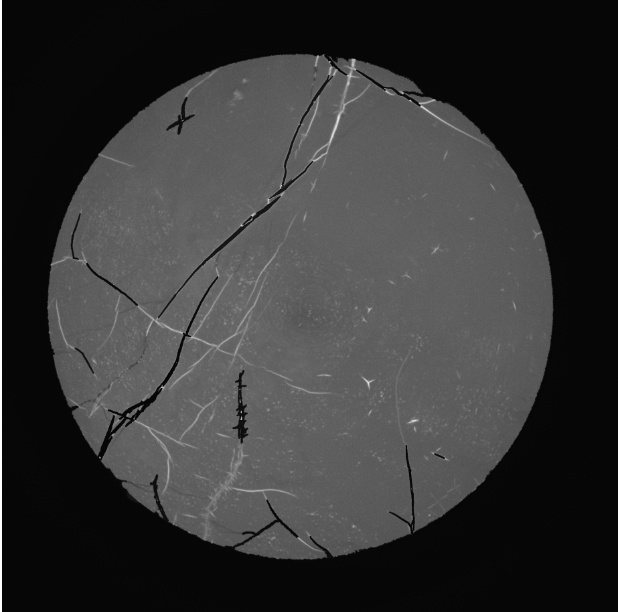
\includegraphics[height=4.0cm]{fig/amostra-carvao.png}} \hspace*{0.1cm}
    \subfloat[]{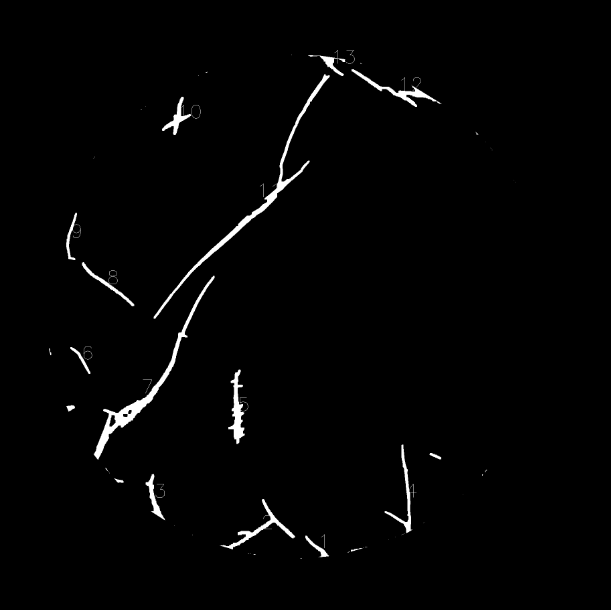
\includegraphics[height=4.0cm]{fig/seg-num.png}}\\
    \scriptsize{Imagens para testes de fraturas. (k) imagem de amostra de carvão com algumas calcificações em preto; (l) resultado da segmentação.}
    \end{figure}
\end{frame}

\begin{frame}{Resultados}{Analise das Características: Fraturas}

\begin{itemize}
    \item Diferentemente da análise anterior, nessa amostra com diferentes tipos de fraturas, nem todas as estruturas foram rotuladas corretamente.
   \begin{itemize}
        \item 77\% de de acerto com relação a caracterização dos tipos.
        \item No calculo do ângulo, as bifurcações presentes nas fraturas trouxeram confusão em 3 classificações. Nesses casos, a inclinação e a bifurcação das fraturas traz uma incerteza à classificação do ângulo.
        \item Na caracterização geral da fatia, 13 fraturas foram identificadas, sendo 2 na vertical e 11 inclinadas, detectando 100\% de fraturas não-sistemáticas, em que o valor correto deveria ser 77\%, pois 3 fraturas possuem características sistemáticas.
   \end{itemize}
   
    \item Todas as fraturas foram caracterizadas com comprimento e largura corretos. 
    \item O único critério que não pôde ser avaliado foi a densidade, pois é um parâmetro que serve de estimativa a segmentação realizada.
\end{itemize}    

\end{frame}

\begin{frame}{Resultados}{Analise das Características: Poros}
    \begin{itemize}
        \item Amostra 1 com 8,024\% de Macroporosidade, poros com uma média de 8,395px de diâmetro, sendo 3994 poros identificados;
        \item Amostra 2 com 1,95\% de Macroporosidade, poros com uma média de 12px de diâmetro, sendo 474 poros identificados;
    \end{itemize}    
        
    \begin{figure}[!htb]
        \centering
        \subfloat[]{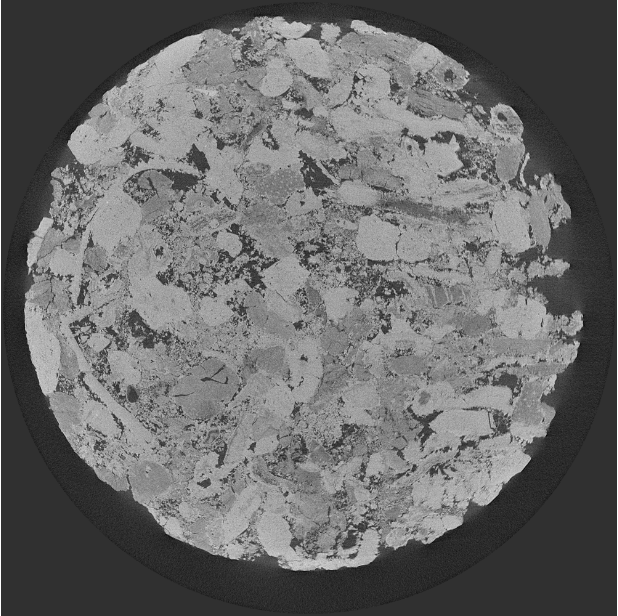
\includegraphics[height=3.0cm]{fig/img_original.png}} \hspace*{0.1cm}
        \subfloat[]{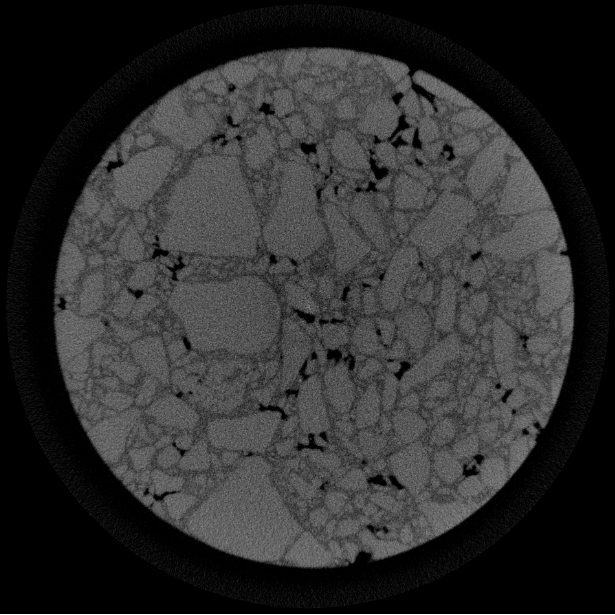
\includegraphics[height=3.0cm]{fig/amostra-2.png}}\\
        \scriptsize{Amostras para análise de porosidade. (m) Amostra 1 (mais porosa) (n) Amostra 2 (menos porosa).}
        \end{figure}
    \end{frame}
    
\begin{frame}{Resultados}{Analise da Segmentação: Dificuldades Encontradas}
    \begin{itemize}
        \item Algumas fraturas não conseguiram ser facilmente extraídas, o que pode ser justificado pela tonalidade e espessura das fraturas, que muitas vezes impedem que o algoritmo de segmentação consiga extrair corretamente todo o corpo da fratura.
    \end{itemize}

    \begin{figure}[!htb]
        \centering
        \subfloat[]{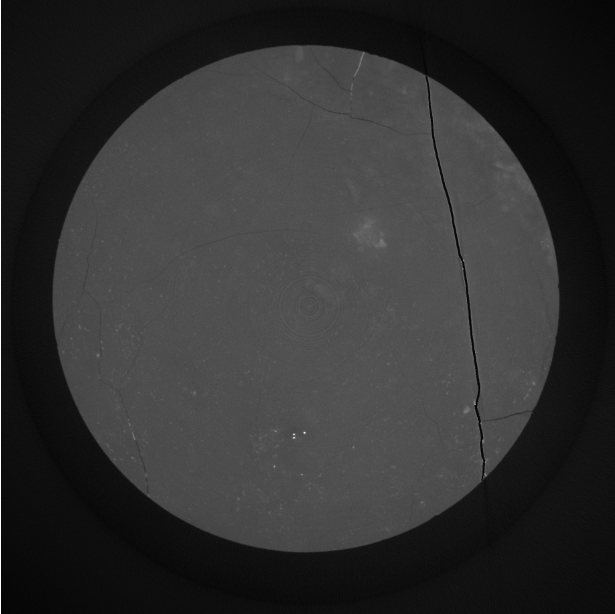
\includegraphics[height=3.0cm]{fig/falha-1.png}} \hspace*{0.1cm}
        \subfloat[]{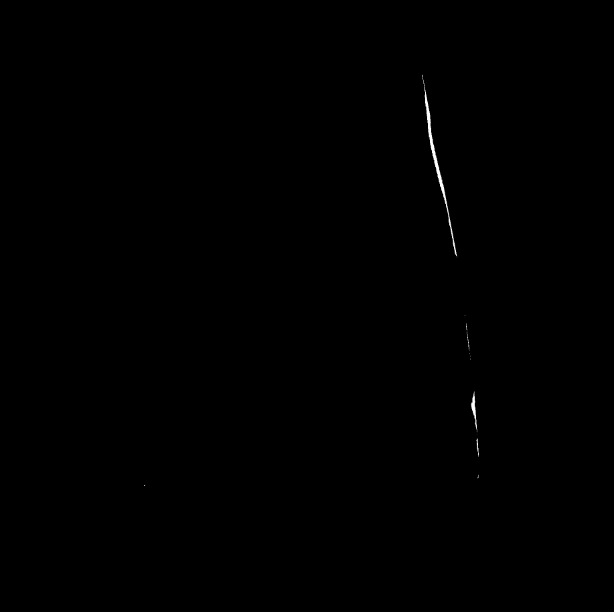
\includegraphics[height=3.0cm]{fig/seg-falha-1.png}}\\
        \scriptsize{Resultado da segmentação de fraturas finas. (o) imagem com fratura sintética; (p) resultado da segmentação.}
    \end{figure}
\end{frame}

\begin{frame}{Resultados}{Ferramenta Desenvolvida: Tela Inicial}
    \begin{itemize}
        \item \textbf{Tela Inicial da Ferramenta:} Possibilita a interação com os dois ambientes.
    \end{itemize}
    
    \begin{figure}[!htb]
    \centering
    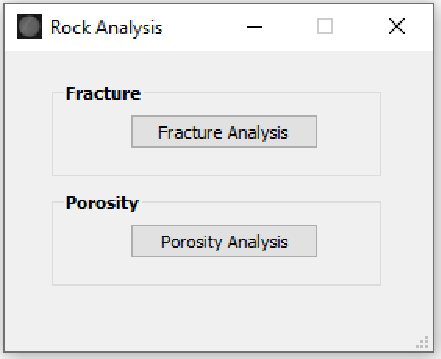
\includegraphics[width=4.5cm]{fig/tela_inicial.pdf}\hspace*{0.1cm}
    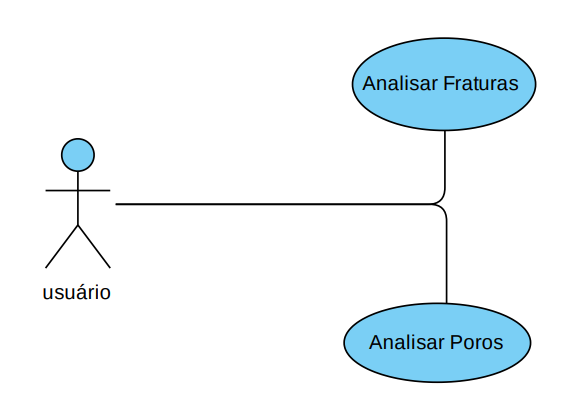
\includegraphics[width=4.5cm]{fig/casos-1.PNG}\\
    \scriptsize{Apresentação da tela inicial da ferramenta desenvolvida e seu Diagrama de Casos de Uso.}
    \label{fig:tela_inicial}
    \end{figure}
\end{frame}


\begin{frame}{Resultados}{Ferramenta Desenvolvida: Tela Fratura}
    \begin{itemize}
        \item \textbf{Tela Fraturas:} Possibilita a interação com os resultados obtidos através das imagens passadas como parâmetro para analisar as fraturas.
    \end{itemize}
    
        
    \begin{figure}[!htb]
    \centering
    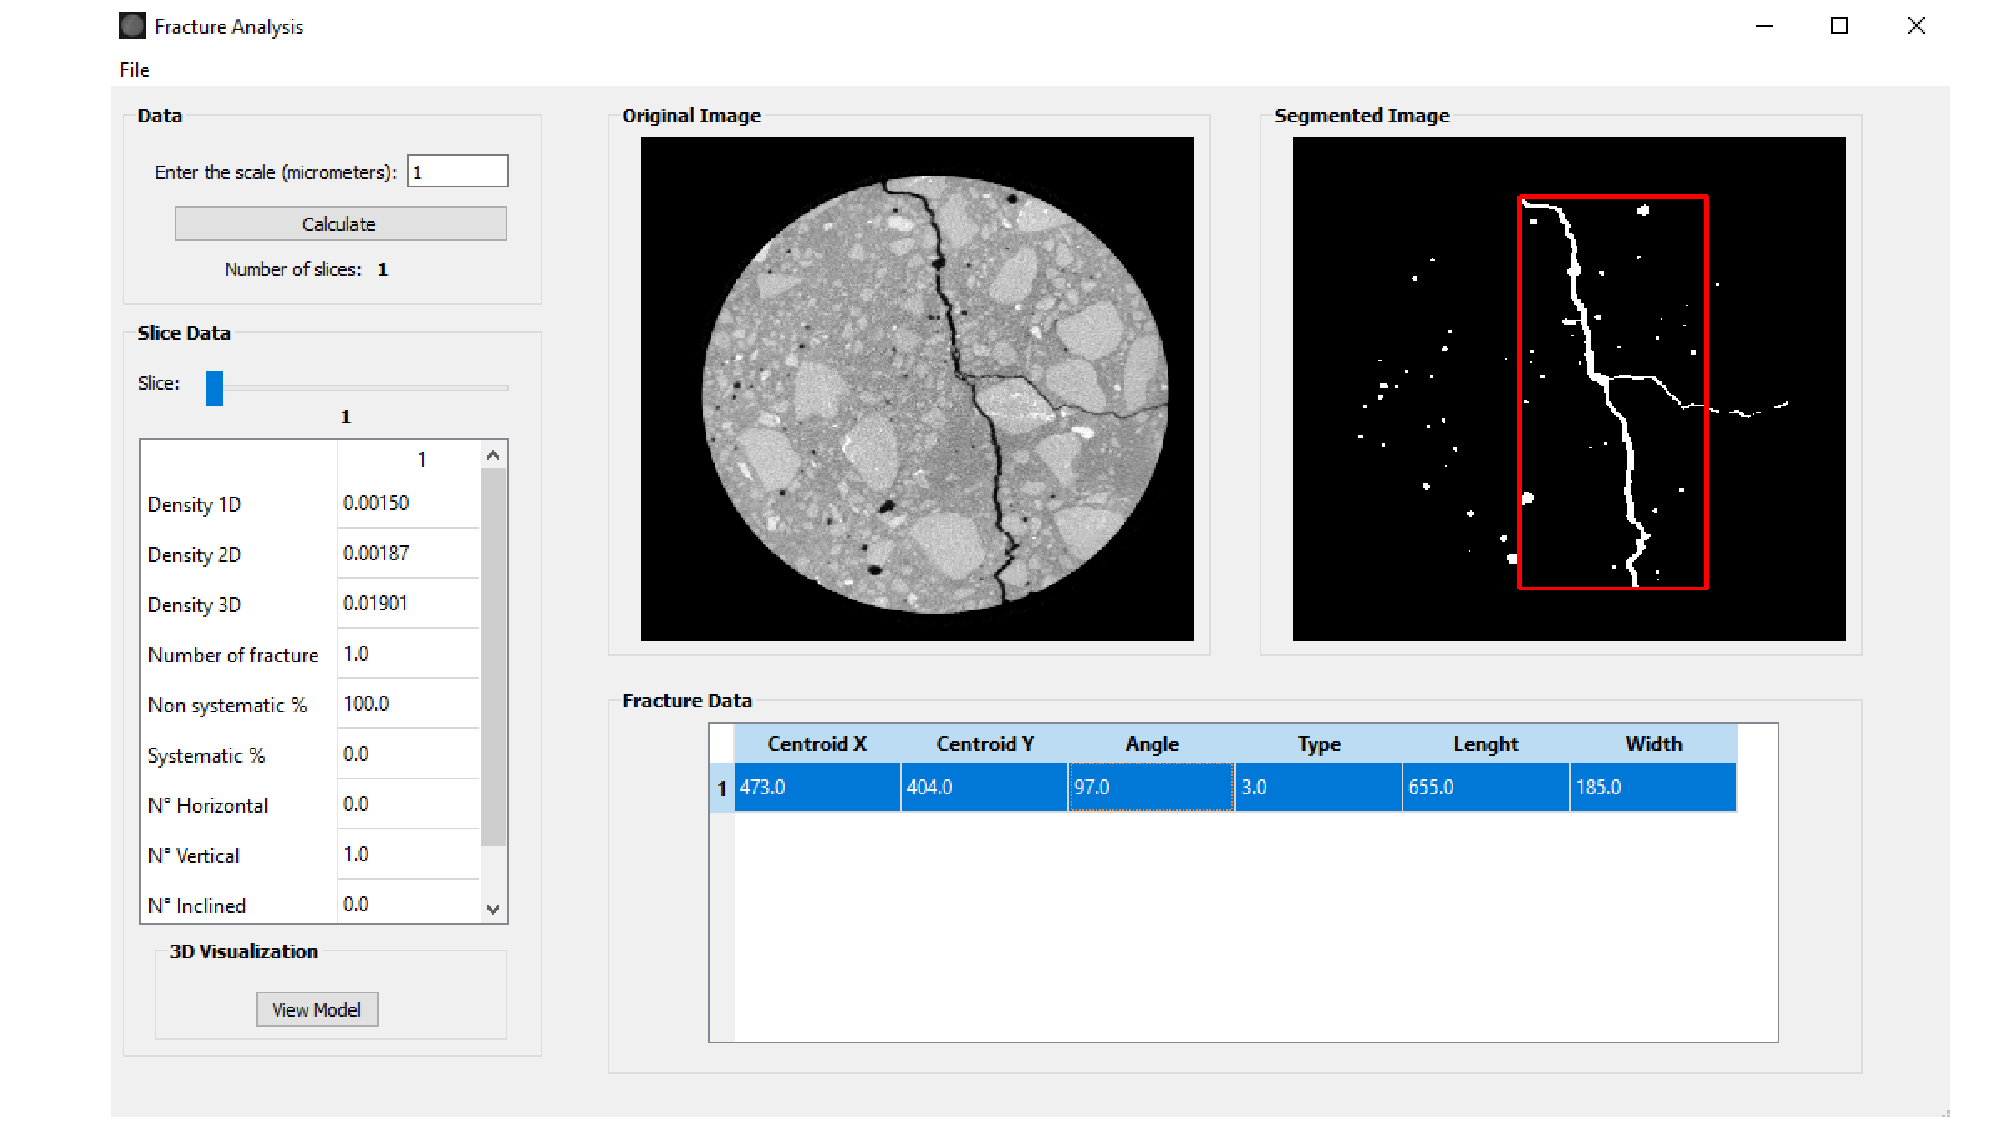
\includegraphics[width=8.5cm]{fig/tela-fracture.pdf}\\
    \scriptsize{Apresentação da tela referente à visualização dos dados das fraturas.}
    \end{figure}
\end{frame}

\begin{frame}{Resultados}{Casos de Uso: Tela Fratura}
        
    \begin{figure}[!htb]
    \centering
    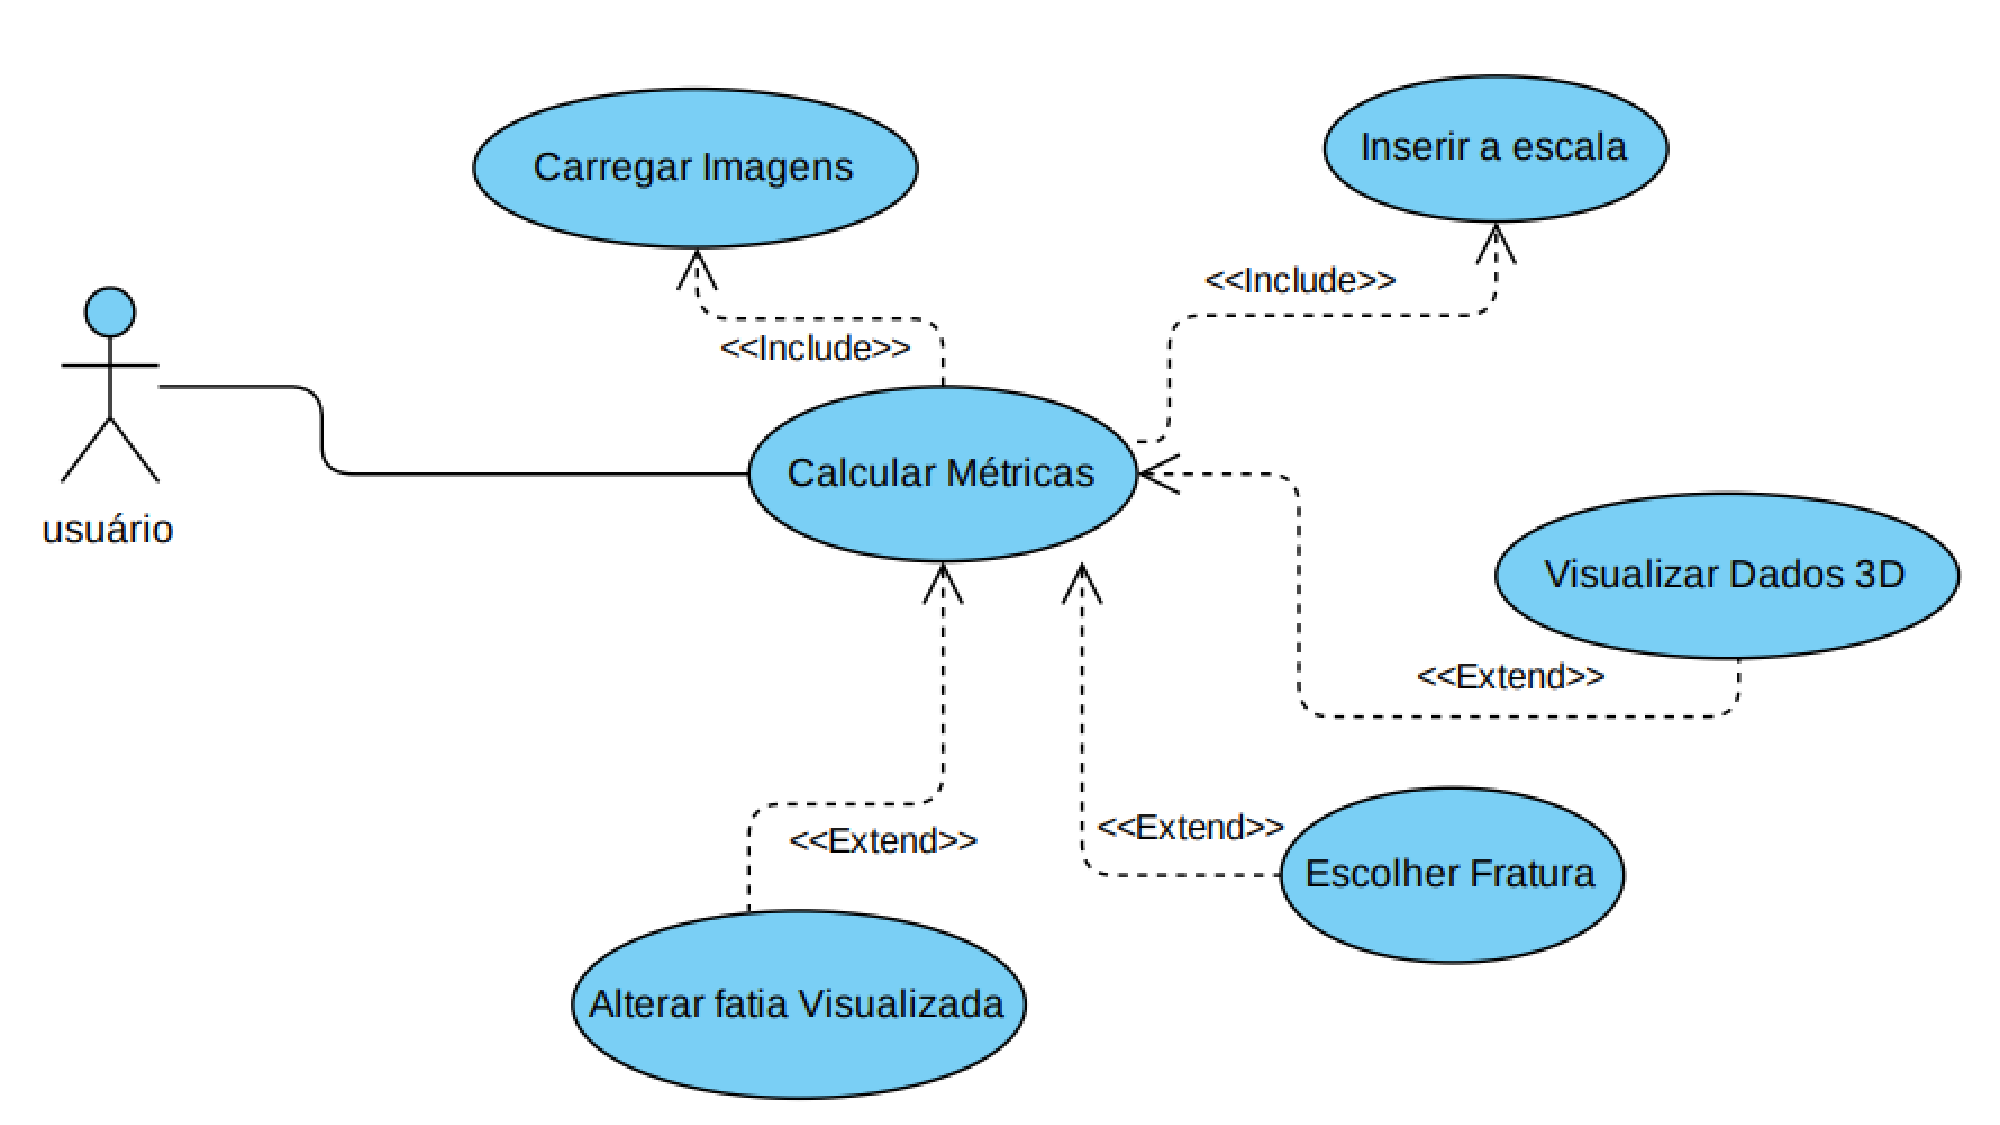
\includegraphics[width=12cm]{fig/casos-2.pdf}\\
    \scriptsize{Diagrama de casos de uso da análise de fraturas.}
    \end{figure}
\end{frame}


\begin{frame}{Resultados}{Ferramenta Desenvolvida: Tela Poros}
    \begin{itemize}
        \item \textbf{Tela Poros:} Possibilita a interação com os resultados obtidos através das imagens passadas como parâmetro para analisar os poros.
    \end{itemize}
          
   \begin{figure}[!htb]
    \centering
    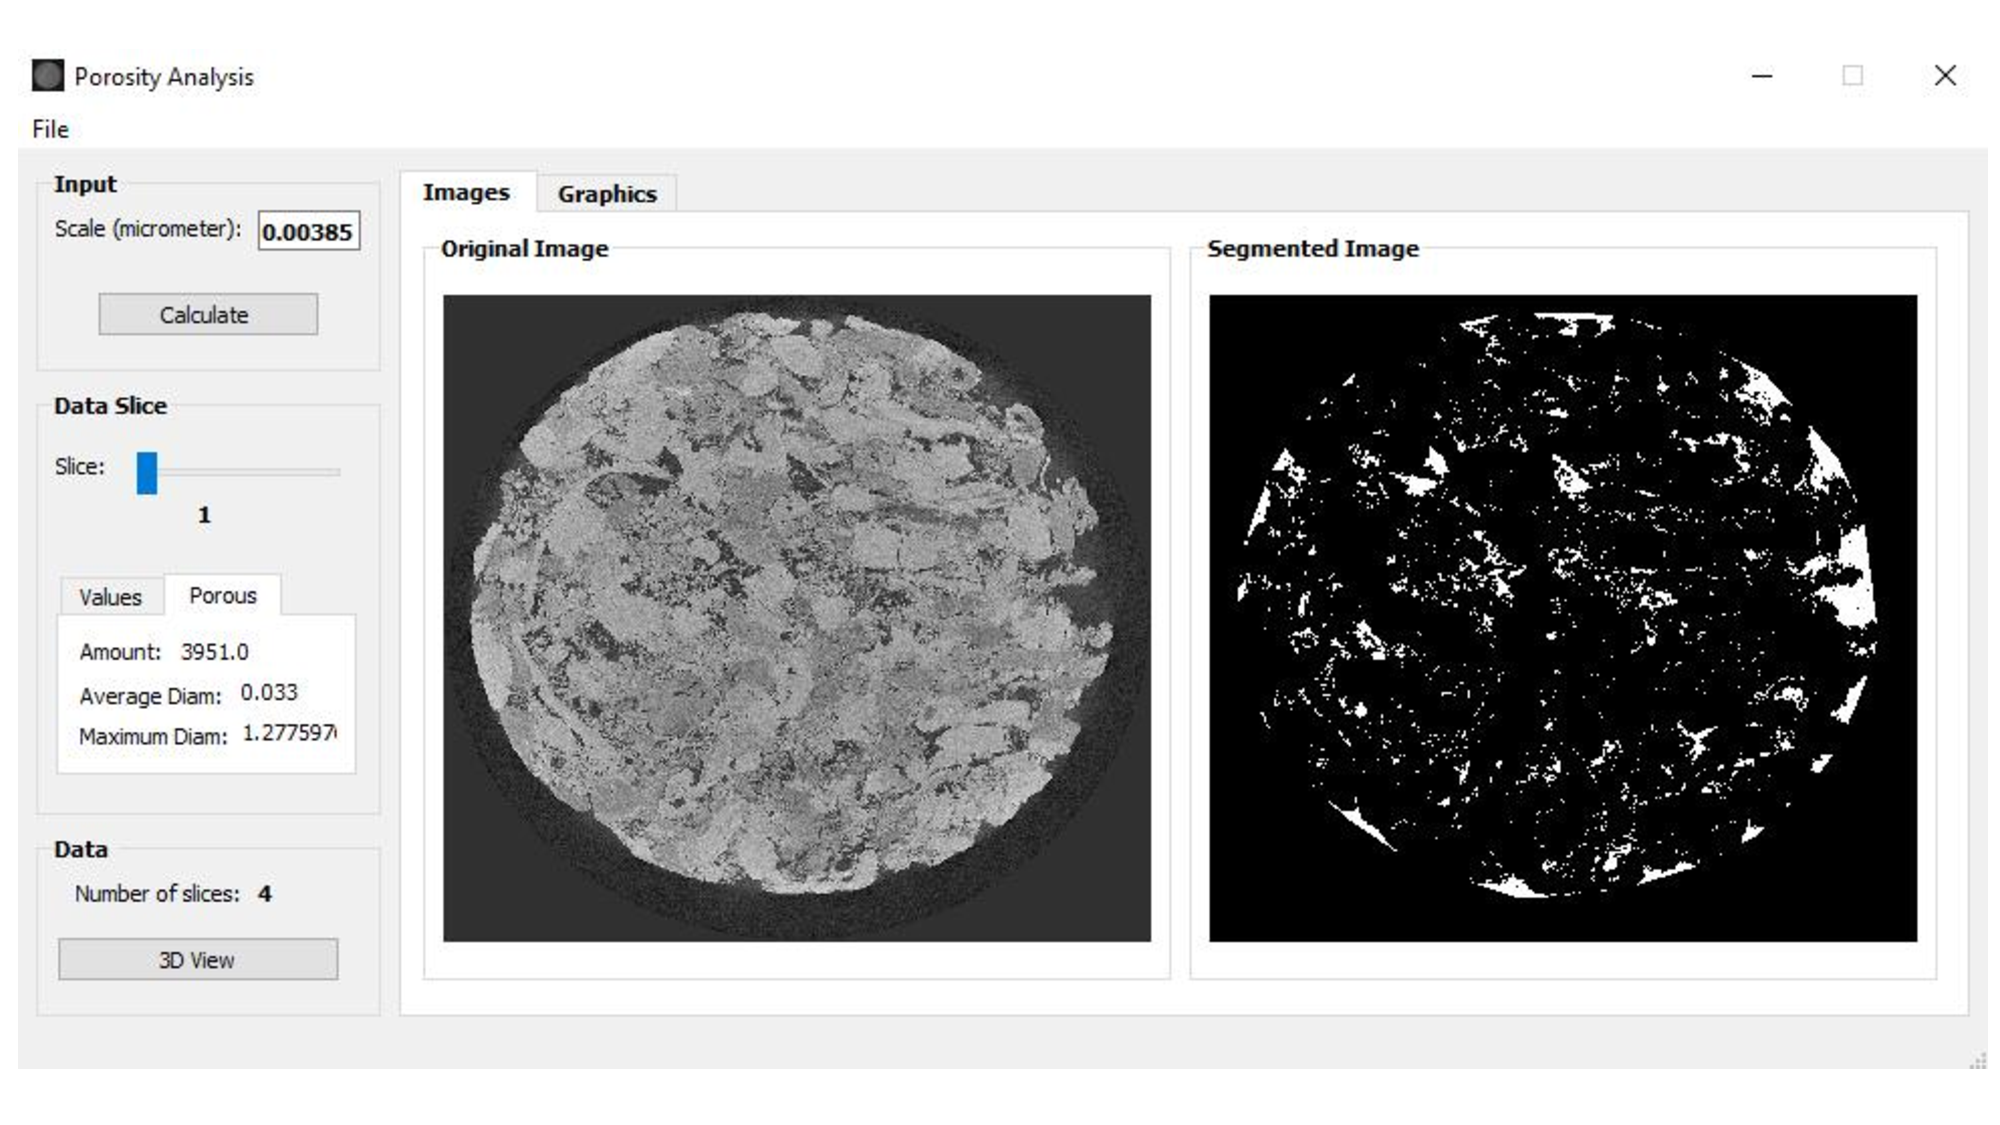
\includegraphics[width=8.5cm]{fig/tela-poro-1.pdf}\\
    \scriptsize{Apresentação da tela referente à visualização dos dados dos poros.}
    \end{figure}
\end{frame}

\begin{frame}{Resultados}{Ferramenta Desenvolvida: Tela Poros}
    
    \begin{figure}[!htb]
    \centering
    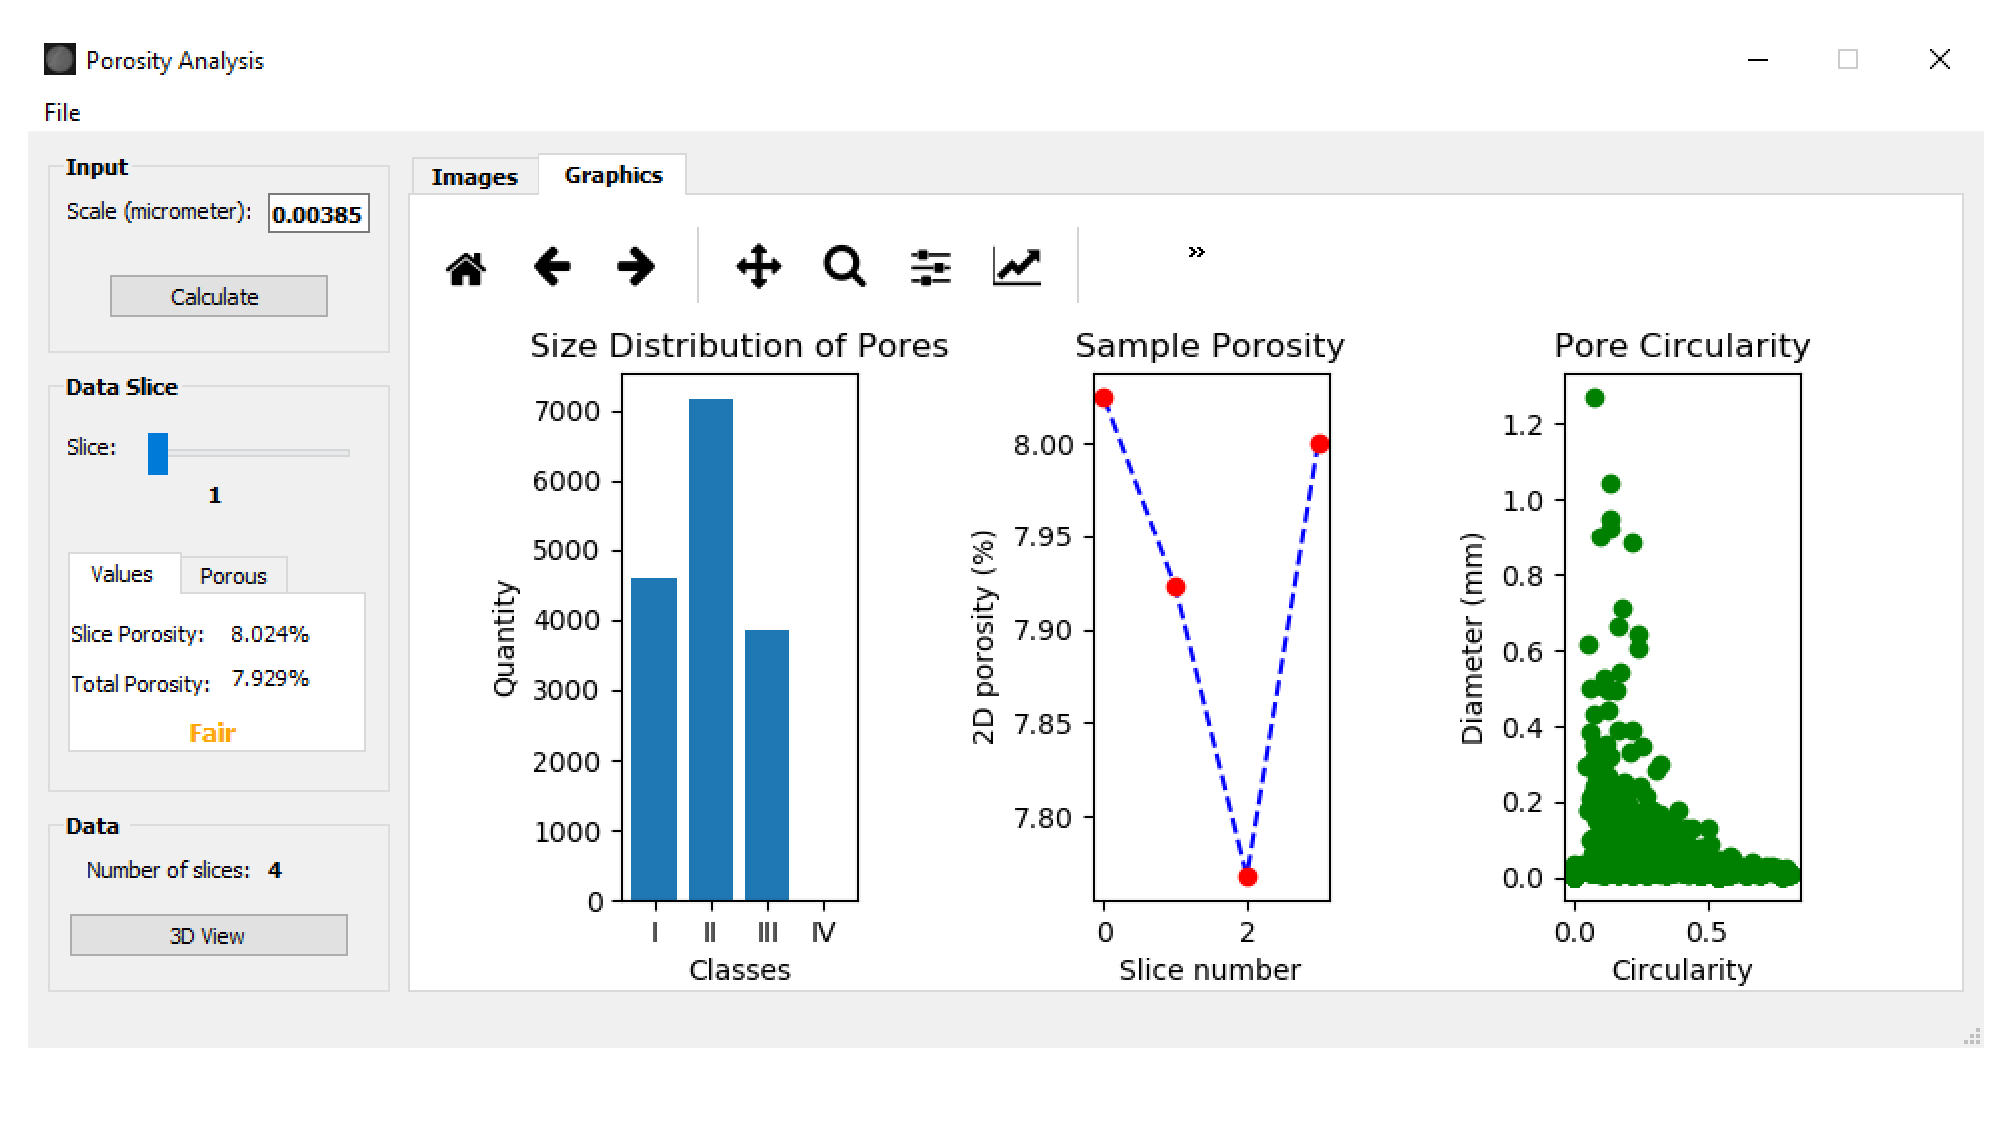
\includegraphics[width=10cm]{fig/tela-poro-2.pdf}\\
    \scriptsize{Apresentação da tela referente à visualização dos gráficos dos poros.}
    \end{figure}
\end{frame}

\begin{frame}{Resultados}{Casos de Uso: Tela Poros}
    \begin{figure}[!htb]
    \centering
    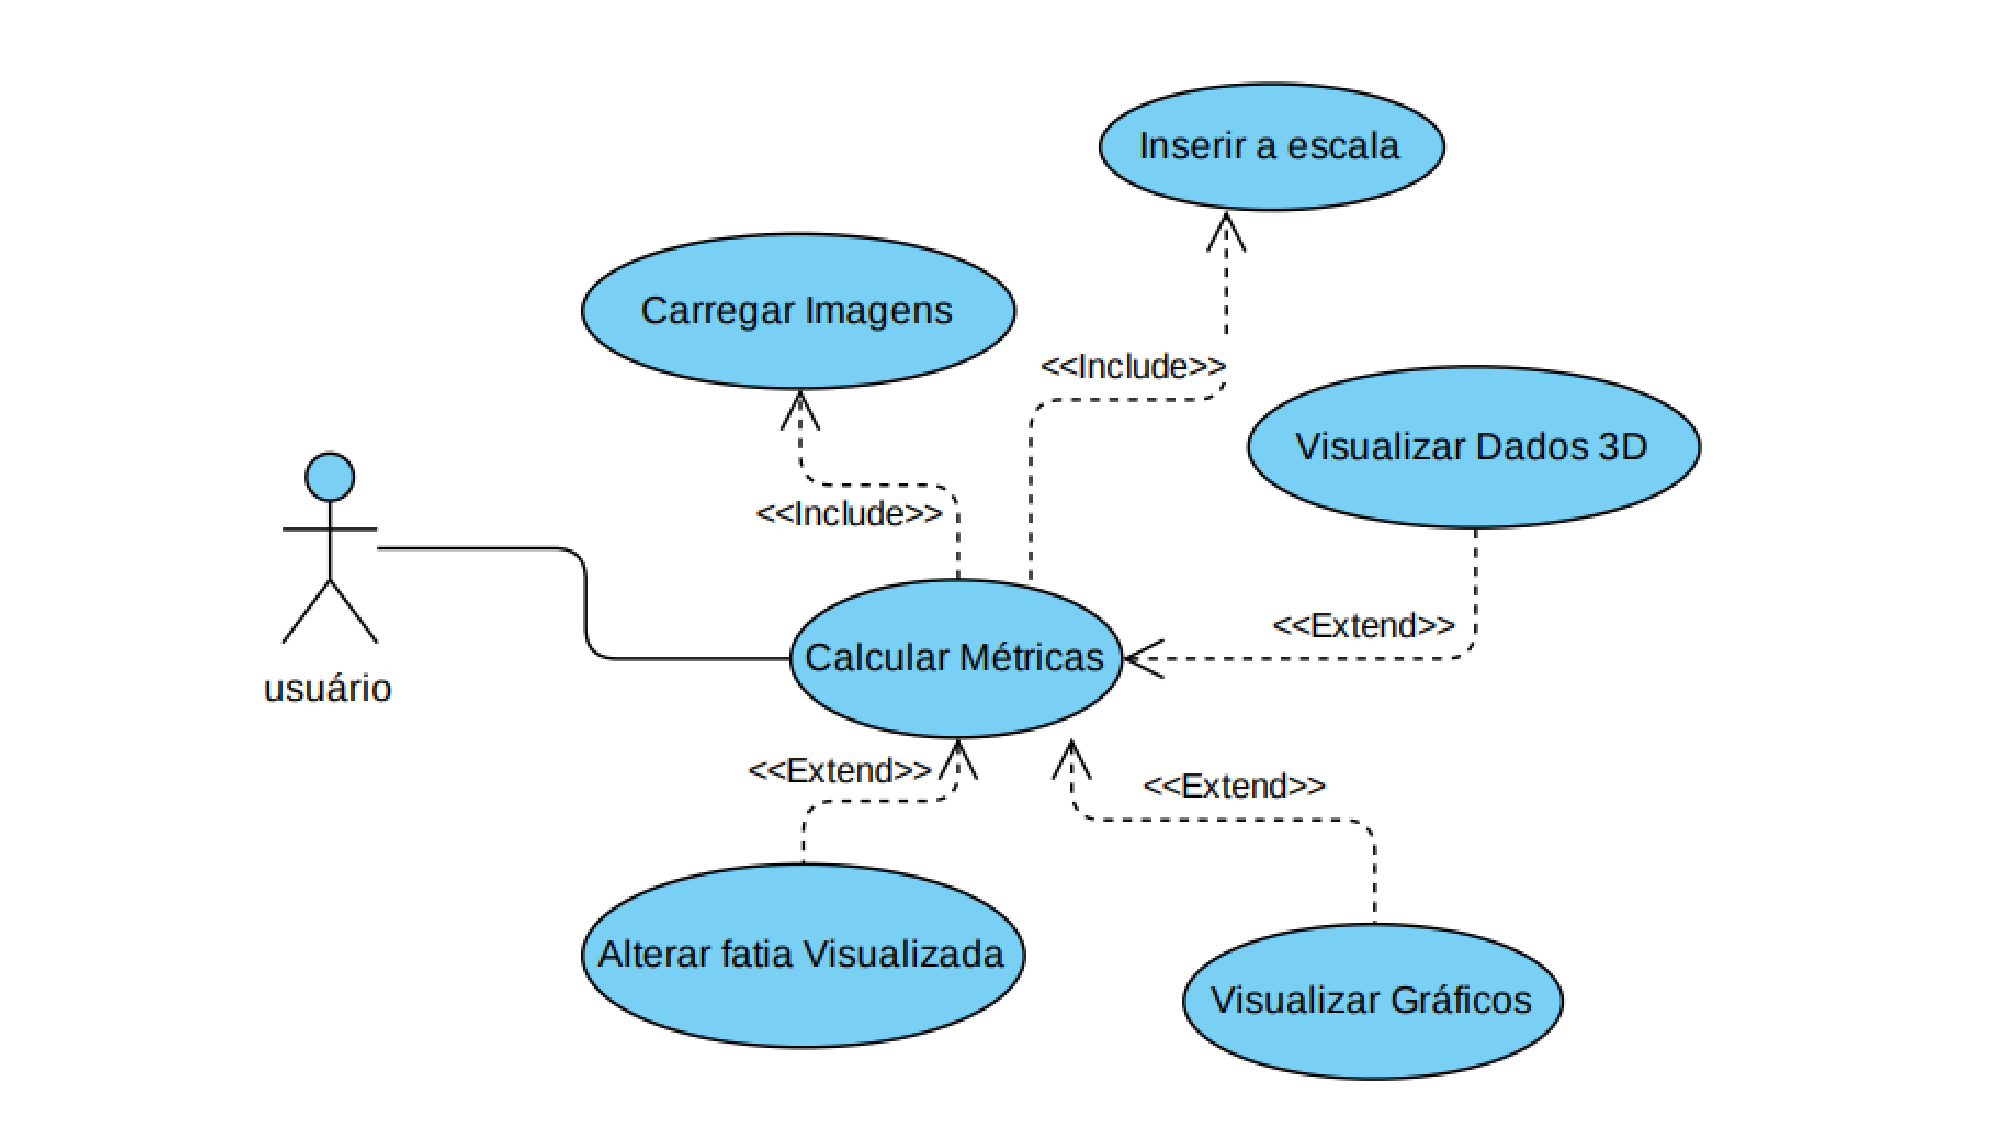
\includegraphics[width=12.0cm]{fig/casos-3.pdf}\\
    \scriptsize{Diagrama de casos de uso da análise de poros.}
    \end{figure}
\end{frame}
\begin{frame}{Resultados}{Visualização 3D}
    
    \begin{itemize}
        \item Resultado das Visualização 3D das amostras porosas.
    \end{itemize}
          
    \begin{figure}[!htb]
    \centering
    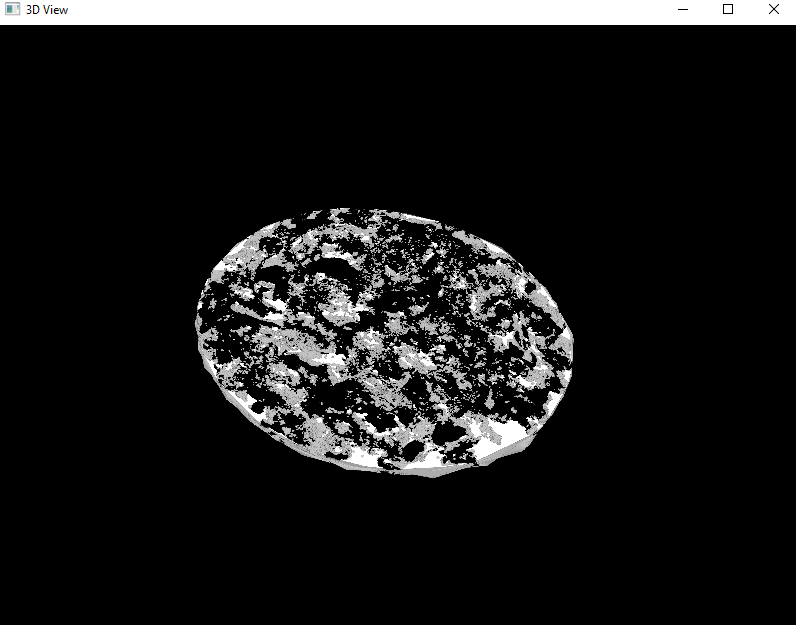
\includegraphics[height=4cm]{fig/3dview-2.png} \hspace*{0.1cm}
    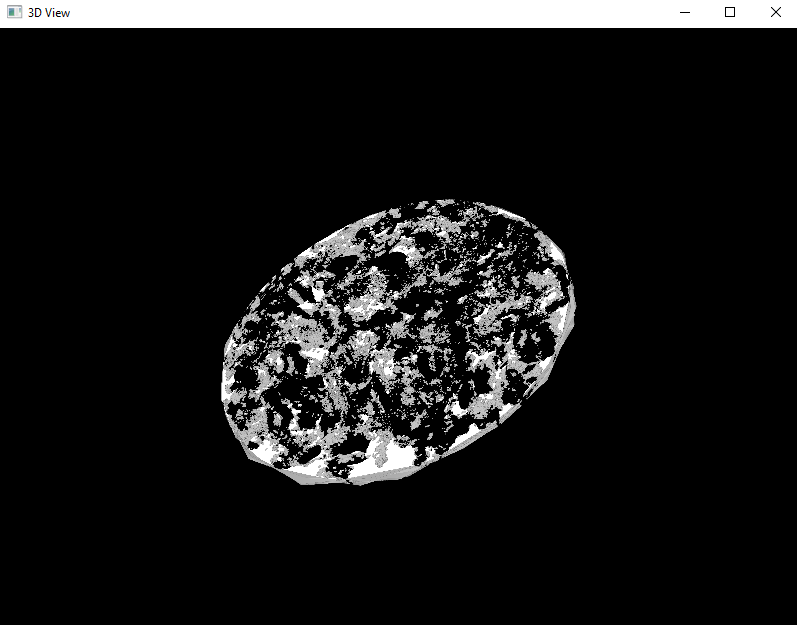
\includegraphics[height=4cm]{fig/3dview-1.png}\\
    \scriptsize{Diferentes visões obtidas da amostra pela tela de visualização 3D dos poros.}
    \end{figure}
\end{frame}

\begin{frame}{Resultados}{Tempo de Execução}
    \begin{itemize}
        \item Elaboramos um conjunto de dados com 12 imagens sintéticas.
        \item Realizamos dois tipos de testes: (i) a análise do tempo de acordo como aumento de fraturas em uma mesma imagem e (ii) a análise do tempo dado o aumento de imagens para uma mesma entrada.
    \end{itemize}
    
\end{frame}


\begin{frame}{Resultados}{Tempo de Execução}
    \begin{figure}[!htb]
    \centering
    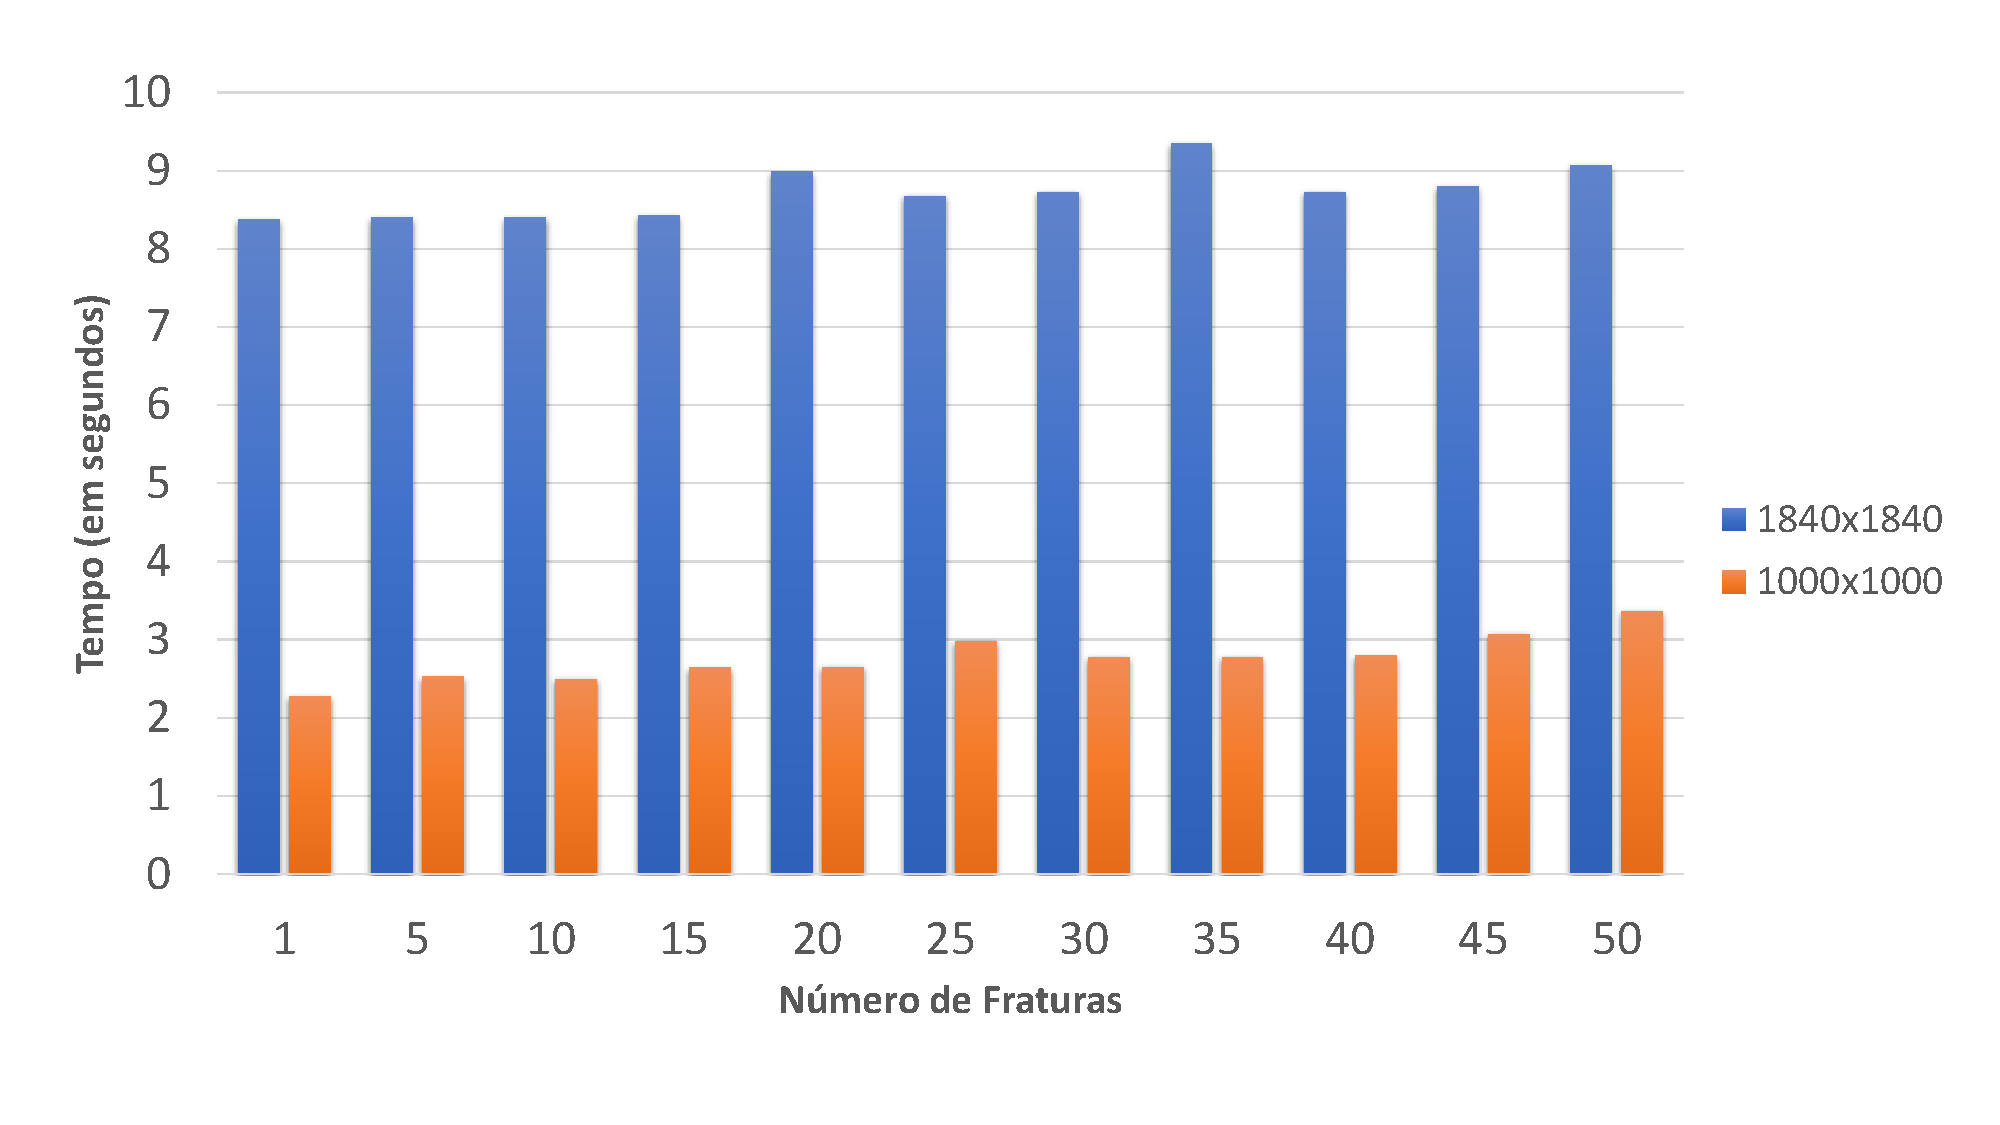
\includegraphics[width=1.\textwidth]{fig/tempo-fraturas.pdf} \\
    \scriptsize{Gráfico do tempo de execução da ferramenta, dado o número de fraturas em uma imagem com imagens de dimensões 1840$\times$1840 e 1000$\times$1000 pixels.}
    \label{fig:graf-tempop1}
    \end{figure}
\end{frame}

\begin{frame}{Resultados}{Tempo de Execução}
        
    \begin{figure}[!htb]
    \centering
    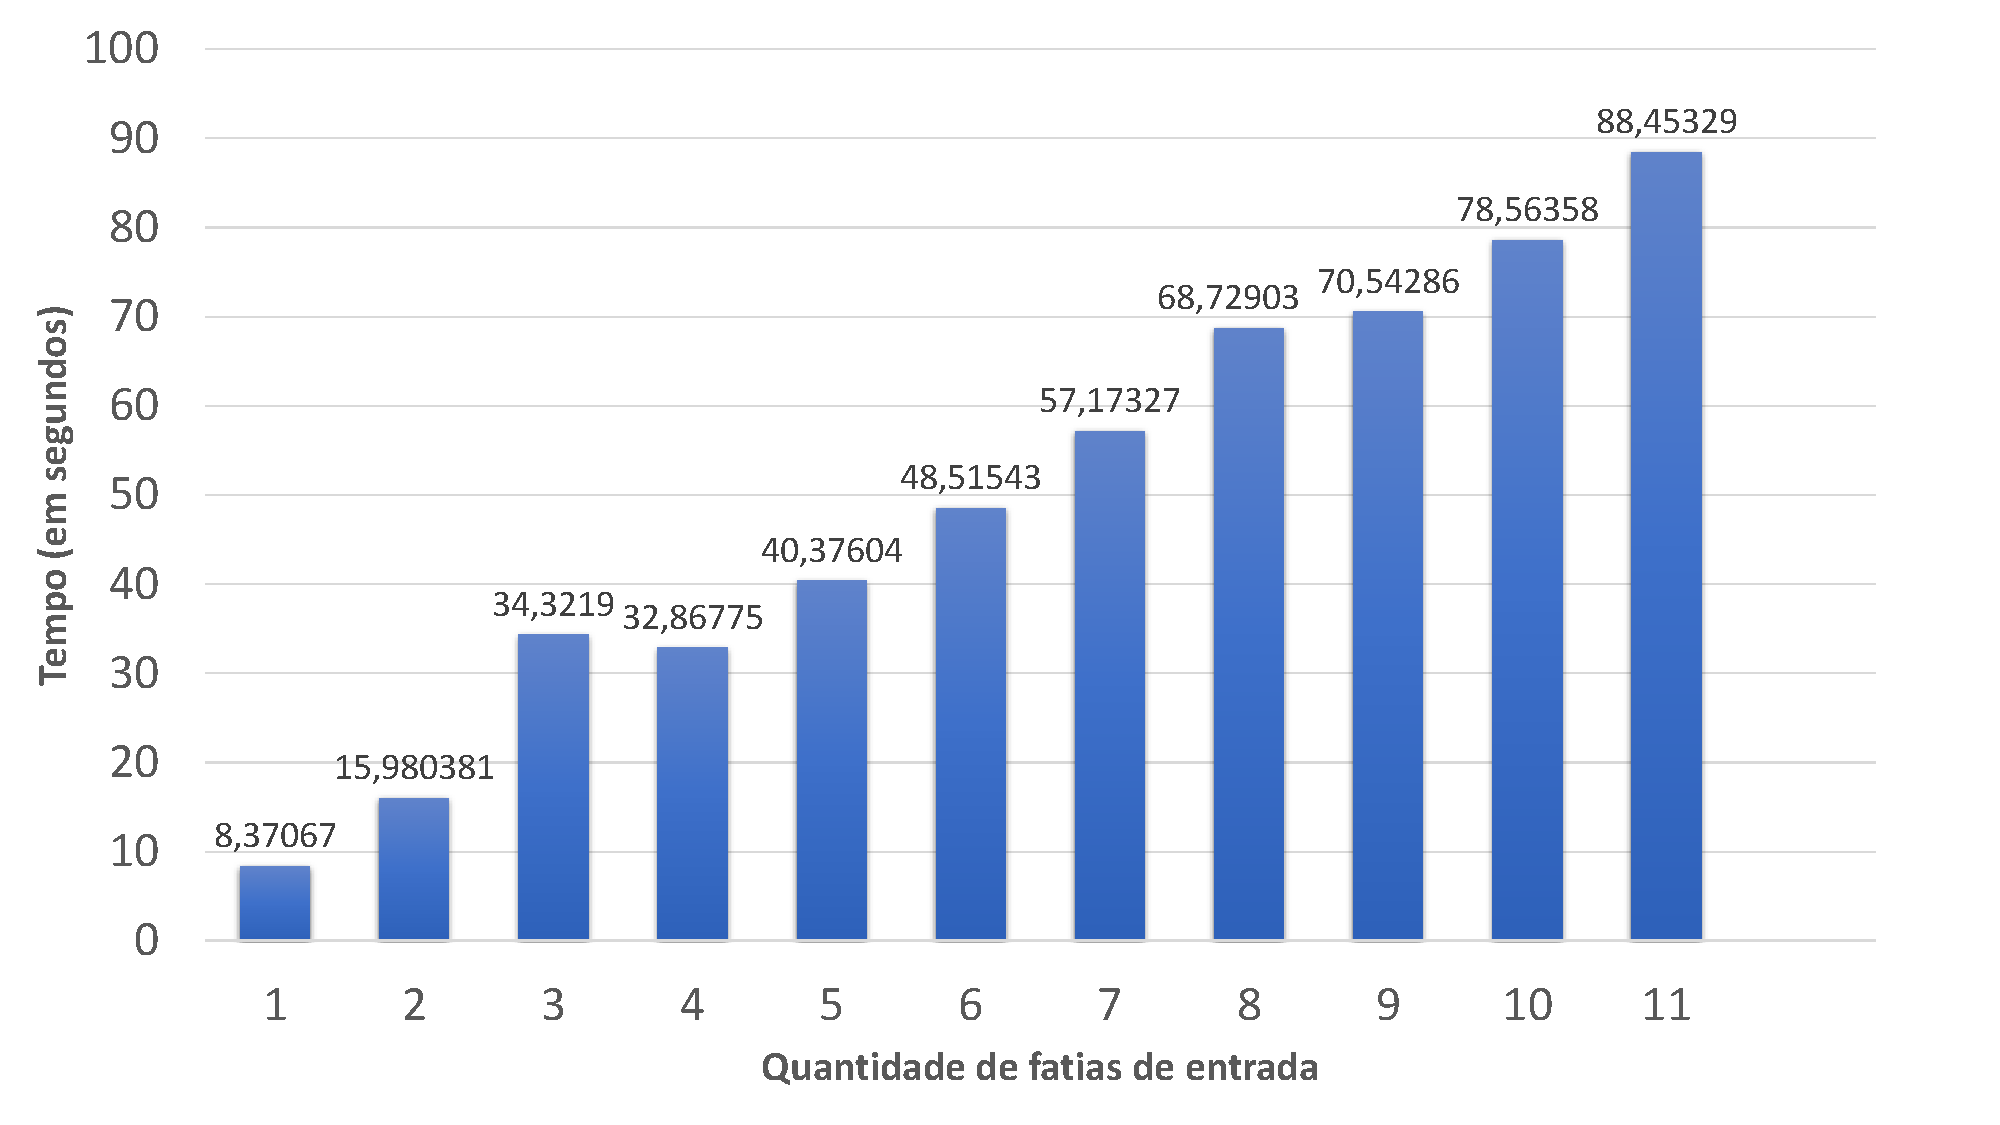
\includegraphics[width=.9\textwidth]{fig/grafico-tempo.pdf}\\
    \scriptsize{Gráfico do tempo de execução da ferramenta, dado o número de fatias de entrada.}
    \end{figure}

\end{frame}

\begin{frame}{Resultados}{Teste de Dimensionalidade}
    
    \begin{table}[!htb]
    \setlength{\tabcolsep}{3.0mm}
    \centering
    \caption{Comparação do tempo de execução (em segundos) de duas amostras com dimensões diferentes.}
    \label{tab:tab_tempo}
    \begin{tabular}{ccc}
    \toprule
    Amostras & \multicolumn{1}{c}{Tamanho}  & \multicolumn{1}{c}{Redimensionada} \\
             & \multicolumn{1}{c}{Original} & \multicolumn{1}{c}{(1000$\times$1000 pixels)} \\
    \midrule
    Amostra 1 (2000x2000) & 60,240s & 11,073s \\
    Amostra 2 (1792x1792) & 36,253s & 11,017s \\
    \bottomrule
    \end{tabular}
    \end{table}
    
    \begin{table}[!htb]
    \setlength{\tabcolsep}{3.0mm}
    \centering
    \caption{Comparação do número de poros detectados.}
    \label{tab:tab_poro}
    \begin{tabular}{ccc}
    \toprule
    Amostras & \multicolumn{1}{c}{Tamanho}  & \multicolumn{1}{c}{Redimensionada} \\
             & \multicolumn{1}{c}{Original} & \multicolumn{1}{c}{(1000$\times$1000 pixels)} \\
    \midrule
    Amostra 1 & 3994 & 1009 \\
    Amostra 2 &  474 &  113 \\
    \bottomrule
    \end{tabular}
    \end{table}
\end{frame}

%-------------------------------
\section{Conclusões}
%-------------------------------

\begin{frame}{Conclusões}
Sendo assim, podemos responder as hipóteses iniciais:
    \item A segmentação por limiarização é suficiente para extrair corretamente as estruturas internas das amostras?
    \begin{itemize}
        \item Não, não foi suficiente para prover uma extração adequada da região de interesse. Por isso, aplicamos o método de \textit{watershed} para extrair a região de interesse, e algumas operações de morfologia matemática para suprir a capacidade de detalhamento na extração.
    \end{itemize}
    
    \item Quais as principais características a respeito da geometria das fraturas? É possível caracterizá-las a partir das estruturas extraídas?
    \begin{itemize}
        \item Conseguimos identificar oito principais características, das estruturas internas à rocha, sendo (i) três a respeito dos poros: porosidade,circularidade e visibilidade e (ii) cinco a respeito das fraturas: número, tamanho, conectividade, orientação e densidade.
    \end{itemize}
\end{frame}

\begin{frame}{Conclusões}
     \item Qual a melhor maneira de interagir com os resultados obtidos pela caracterização?
    \begin{itemize}
        \item Desenvolvemos uma ferramenta interativa que se mostrou uma maneira adequada de interagir com os resultados obtidos pelo algoritmo desenvolvido.
    \end{itemize}
    
    \item Outras conclusões:
    \begin{itemize}
        \item A segmentação mostrou-se a principal etapa para a classificação das estruturas.
        \item Redimensionar a imagem pode excluir o benefício que a técnica de microtomografia oferece.
        \item O tempo de execução da ferramenta está diretamente ligado a quantidade de imagens de entrada. Ou seja, é inviável o trabalho com todas as imagens correspondentes à amostra.
    \end{itemize}
\end{frame}

\begin{frame}{Conclusões}{Trabalhos Futuros}
    \begin{itemize}
        \item Aprimoramento dos métodos de segmentação das imagens de MicroCT.
        \item Desenvolvimento de bases de dados artificiais baseados do métodos de \textit{Machine Learning}.
        \item Atualmente um artigo com os resultados da pesquisa está em fase final de produção.
    \end{itemize}
\end{frame}

\begin{frame}{Agradecimentos}
    \item À banca presente.
    \item Ao meu orientador, Hélio Pedrini, e ao Co-orientador, Guilherme Avansi.
    \item Aos amigos e familiares.
    \item Ao Instituto de Computação da UNICAMP e a seus funcionários.
    \item À Fundação de Amparo à Pesquisa do Estado de São Paulo (FAPESP), processo 2017/50065-2, com o autor sob processo 2018/01439-0, e à Coordenação de Aperfeiçoamento de Pessoal de Nível Superior (CAPES), processo sob número 88887.363636/2019-00, pelo apoio financeiro.
\end{frame}
\end{document}